\documentclass[a4paper,11pt]{article}
\usepackage[utf8]{inputenc}
\usepackage[francais]{babel}
\usepackage[T1]{fontenc}

\usepackage[toc,page]{appendix}
%fonts pour les math
\usepackage{amsfonts}
\usepackage{amsmath}
\usepackage{dsfont}
\usepackage{stmaryrd}
%couleur dans le doc
\usepackage[dvipsnames]{xcolor}
\usepackage{ulem}
%\usepackage{lastpage}
%pour les images
	\usepackage[dvips, pdftex]{graphicx}
	\usepackage[section]{placeins}
	\usepackage{here}
	\usepackage{float}

%définition du titre du document
\newcommand{\titleinfo}{\textcolor{MidnightBlue}{MEC431 – Projet}}
 %\newcommand{\sectionprefix}{Q}

\usepackage{tikz}
\usepackage{url}
%\usepackage{hyperref} On n'a pas besoin pour le moment
%\usepackage{pst-plot}
%\usepackage{pst-grad}
%\usepackage{pst-node}
\usepackage{booktabs}
%formattage de la page
	\usepackage{geometry}
	\geometry{top=2cm, bottom=2cm, left=2cm, right=2cm}
	%fomattage de l'entête et du pied de page
	\usepackage{fancyhdr}
		\setlength{\headheight}{15.2pt}
		\lhead{\titleinfo}
		\rhead{\leftmark}
	\pagestyle{fancy}


%formattage du titre des sections
	%\usepackage{titlesec}
	%\titleformat{\section}[runin]{\normalfont\bfseries}{\sectionprefix \thesection}{1pt}{}[.]

%longueur des sauts de paragraphe
\setlength{\parskip}{1ex}

%commande pour les ensembles
\newcommand{\R}{\mathbb{R}}
\newcommand{\N}{\mathbb{N}}
\newcommand{\C}{\mathbb{C}}

%commande pour les notations de map
	%\newcommand{\I}{\mathds{1}}
	%\newcommand{\p}{\mathds{P}}
	%\newcommand{\E}{\mathds{E}}
	%\renewcommand{\P}{\mathds{P}}

%pour les transposées
\usepackage{tensor}

\newcommand{\trans}[1]{\tensor[^t]{#1}{}}

%commande pour les opérateurs
\newcommand{\INT}{\displaystyle\int}
\newcommand{\SUM}{\displaystyle\sum}
\newcommand{\FRAC}{\displaystyle\frac}
\newcommand{\PROD}{\displaystyle\prod}
\newcommand{\INF}{\displaystyle\inf}

\newcommand{\tens}{\uuline}
\newcommand{\verseur}[1]{\uline{e}_{#1}}
\newcommand{\diage}[1]{\uline{e_{#1}} \otimes \uline{e_{#1}}}
\newcommand{\diveleme}[3]{\FRAC{\partial #1_{#2#3}}{\partial #3} e_{#2}}
\newcommand{\dive}{\mathop{\rm div}}
\newcommand{\grad}{\mathop{\rm grad}}

\renewcommand{\theequation}{\Alph{equation}}

% Pour créer des afterpage près des larges images
\usepackage{afterpage}
\setlength\fboxrule{0.6pt}% pour donner plus d'importance a la boite qui entoure resultat final


\begin{document}
\title{\titleinfo}
\author{
	François \bsc{Espinet}
	\\
	Thomas \bsc{Ferreira de lima}
	\\
	Sophie \bsc{Rousselle}
	\\
	Oscar \bsc{Flores Altamirano}
}
\date{}
\maketitle

\section{Calcul de structure}

\subsection{Données du problème}

\begin{itemize}
\item géométrie initiale:
Cylindre de section droite circulaire, de rayon intérieur A et d'épaisseur E, délimité par 2 plans perpendiculaires à l'axe
\item cinématique imposée:
Origine et directrice fixes, déplacement donné par les surfaces $S_{0}$,  $S_H$, $S_{int}$, $S_{ext}$
\item efforts imposés:
	\begin{itemize}
	\item L'effort volumique est nul car on néglige le poids du système.
	\item Sur la paroi interne $S_{int} (R=A)$:  $\uline{T_d} = -p_i \uline{n}$ et $\uline{n} =- \uline{e_r}$
	\item Sur la paroi externe $S_{ext} (R=A+E)$:  $\uline {T_d} = -p_e \uline{n}$ et $\uline{n} = \uline{e_r}$
	\item sur $S_H (Z=H)$ : $\uline{T_d} = \frac{T}{S_H}\uline{n}$ et $\uline{n} = \uline{e_z}$ (en négligeant l'épaisseur devant le diamètre)
	\end{itemize}
\item comportement: le matériau est élastomère isotrope avec liaison interne et isochorie, donc sa loi de comportement est:
\begin{center}
$$
\tens{\sigma}=2\rho_0\frac{\partial\psi}{\partial I_1}(I_1,I_2)\tens{B} -2\rho_0\frac{\partial\psi}{\partial I_2}(I_1,I_2) \tens{B}^{-1}+q\mathds{1}$$
\end{center}
où :
\begin{flushleft}
$\rho_0$ est la masse volumique;\\
$\psi$ est l'énergie libre massique fonction de la déformation de Green-Lagrange \tens{e} au travers de ses deux premiers invariants $I_1= tr(\tens{B})$ et $I_2=\frac{1}{2}({I_1}^2-\tens{C}:\tens{C})$ et $\tens{C} = {}^t\tens{F}.\tens{F}$ où \tens{F} est le gradient de la transformation;
\\
$q$ est un champ scalaire associé à la liaison d'isochorie.
\end{flushleft}
\end{itemize}

\subsection{Méthode des déplacements}
On suppose que la transformation $\phi : M(R,\Theta, Z) \rightarrow m(r, \theta, z)$ est de la forme:

$$r=\beta(R)R, \theta=\Theta, z=\mu Z$$

\begin{flushleft}
où\\
$\beta(R)>1$ est une fonction de R;\\
$\mu>1$ est une constante.
\end{flushleft}

Comparaison de cette transformation à la structure après transformation:
\begin{itemize}
\item Pour tout point $M(0, \Theta, Z)$ de l'axe $(0z)$, $\phi(M) = m(0, \theta, \mu Z)$ : $m$ appartient à $(Oz)$ donc l'axe $(Oz)$ reste fixe.
\item $\phi (0, 0, 0) = (0, 0, 0)$ donc l'origine $O(0, 0, 0)$ reste fixe.
\item Pour tout point $M(R, \Theta, H)$,  $\phi(M) = m(\beta (R) R, \Theta, \mu H)$ Ainsi le cylindre a une longueur $\mu H$ après transformation.
\item Pour tout point $M(A, \Theta, Z)$ de la paroi interne du cylindre, $\phi(M) = m(\beta(A) A, \theta, \mu Z)$ or la paroi interne après transformation a pour rayon $\lambda A$ d'où
\begin{equation}
\beta(A) = \lambda
\label{eq:condition_limite_beta}
\end{equation}
\item Pour tout point $M(A+E, \Theta, Z)$ de la paroi externe du cylindre, $\phi(M) = m(\beta(A+E) (A+E), \Theta, \mu Z)$ or la paroi externe après transformation est de rayon $\lambda A + e$ d'où :
$$\beta(A+E)(A+E) = \lambda A+ e$$
\end{itemize}
donc cette transformation convient.

Calcul du gradient de transformation :
$$
\begin{array}{rcl}
\tens{F} &=& \tens{grad} \left(\uline{\phi}\right)\\
&=& \left(R\frac{d\beta}{dR} +\beta(R)\right) \uline{e_r}\otimes \uline{e_R} + \beta(R)\ \uline{e_\theta}\otimes \uline{e_\Theta} + \mu\ \uline{e_z}\otimes \uline{e_Z}
\end{array}
$$
On peut remarquer qu'on a : $\uline{e}_{R} = \uline{e}_{r}$, $\uline{e}_{\Theta} = \uline{e}_{\theta}$ et $\uline{e}_{Z} = \uline{e}_{z}$ d'après la transformation choisie. Dans ce cas, l'expression du gradient se simplifie en :

\begin{equation}
\fbox{$
\tens{F} =  \left(R\frac{d\beta}{dR} +\beta(R)\right) \diage{r} + \beta(R)\ \diage{\theta} + \mu\ \diage{z}
$}
\label{eq:exp_tenseur_compliquee}
\end{equation}

\subsection{Condition d'isochorie}
La transformation est isochore (volume constant) donc :

\begin{eqnarray*}
det( \tens{F}) &=& 1\\
\left(R \frac{d\beta(R)}{dR} + \beta(R)\right)\cdot \beta(R) \cdot \mu &=& 1\\
\frac{d (R \beta(R))}{dR} \beta(R) &=& \frac {1}{\mu}\\
\frac{d (R \beta(R))}{dR} R\beta(R) &=& \frac {R}{\mu}\\
R\beta(R) d(R\beta(R)) &=& \frac{R}{\mu} dR\\
\frac{(R\beta(R))^2}{2} &=& \frac{R^2}{2\mu}+K\\
\end{eqnarray*}

où K est une constante. Or d'après \ref{eq:condition_limite_beta}, $\beta(A) = \lambda$, d'où

\begin{eqnarray*}
\frac{A^2\lambda^2}{2} = \frac{A^2}{2\mu}+K &\Longrightarrow& K = \frac{A^2}{2}\left(\lambda^2-\frac{1}{\mu}\right)\\
\frac{R^2 \beta^2(R)}{2} &=& \frac{R^2}{2\mu}+\frac{A^2}{2}\left(\lambda^2 - \frac{1}{\mu}\right)\\
\beta(R) &=& \sqrt{\frac{1}{\mu}+ \frac{A^2}{R^2}\left(\lambda^2 - \frac{1}{\mu}\right)}\\
\end{eqnarray*}

\subsection{Développment limité au premier ordre de $\beta$}

$\beta$ est liée a $\delta$ de la façon suivante :

\begin{center}
\begin{displaymath}
\begin{array}{rll}

& \beta^2 & = \FRAC{1}{\mu}+\frac{1}{\left(1+\delta\right)^2}\left(\lambda^2-\frac{1}{\mu}\right)  \\
&  & \displaystyle \approx  \frac{1}{\mu}+\left(1-2\delta\right)\left(\lambda^2-\frac{1}{\mu}\right) \\
\Rightarrow & \beta & \displaystyle \approx \left[\frac{1}{\mu} + \left(1-2\delta \right)\left(\lambda^2 -\frac{1}{\mu} \right) \right]^{\frac{1}{2}} \\
& &\displaystyle \approx \lambda\left[1+\left(\frac{1}{\lambda^2\mu}-1 \right)\delta \right]\\
\end{array}
\end{displaymath}
\end{center}

Comme $\delta \ll 1$ on peut prendre $\beta=\lambda$ et on trouve (en injectant dans \ref{eq:exp_tenseur_compliquee})

$$
\uline{\uline{F}} = \frac{1}{\lambda\mu}\uline{e}_r\otimes\uline{e}_R+\lambda\uline{e}_\theta\otimes\uline{e}_\Theta+\mu\uline{e}_z\otimes\uline{e}_Z $$
En effet,
$\left(R \FRAC{d\beta(R)}{dR} + \beta(R)\right)\cdot \beta(R) \cdot \mu = 1$ d'où :
$$
\left(R \frac{d\beta(R)}{dR} + \beta(R)\right) = \frac{1}{\beta(R) \mu} = \frac{1}{\lambda \mu}
$$
Ce qui donne :

$$ \frac{e}{E} = \frac{1}{\lambda\mu} \Longrightarrow \frac{e}{a} = \frac{1}{\lambda\mu} \cdot \frac{E}{\lambda A} = \frac{ \epsilon}{\lambda^2 \mu} \hspace{1cm} \fbox{$\FRAC{e}{a} = \FRAC{\varepsilon}{\lambda^2 \mu}$ }
$$


\subsection{Les invariants de la transformation}
On fait le calcul directement:
$$I_1=\text{tr}\left(\uline{\uline{B}}\right) = \text{tr}\left(\uline{\uline{F}}\cdot{}^{t}\uline{\uline{F}}\right) = \text{tr}\left(\frac{1}{\lambda^2\mu^2}\uline{e}_R\otimes\uline{e}_R + \lambda^2\uline{e}_\Theta\otimes\uline{e}_\Theta + \mu^2\uline{e}_Z\otimes\uline{e}_Z \right)=\fbox{$\left(\FRAC{1}{\lambda\mu}\right)^2+\lambda^2+\mu^2 = I_1$}$$

$$I_2 = \frac{1}{2}\left(I_1^2+\text{tr}\left(\uline{\uline{B}}\cdot\uline{\uline{B}}\right)\right) = \frac{1}{2}\left(I_1^2+\text{tr}\left( \frac{1}{\lambda^4\mu^4}\uline{e}_R\otimes\uline{e}_R + \lambda^4\uline{e}_\Theta\otimes\uline{e}_\Theta + \mu^4\uline{e}_Z\otimes\uline{e}_Z \right)\right)  = \fbox{$\FRAC{1}{\mu^2}+\frac{1}{\lambda^2}+\lambda^2\mu^2 = I_2$}$$


\subsection{Calcul de la contrainte de Cauchy}

L'hypothèse $\sigma_{rr} \ll \sigma_{\theta\theta}$, en utilisant l'équation (1) de l'énoncé, aboutit à la relation suivante puisque $\tens{\sigma} = \tens{\sigma'} + q \mathds{1}$:

$$\sigma_{\theta\theta} - \sigma_{rr} = \sigma'_{\theta\theta} - \sigma'_{rr} \approx \sigma_{\theta\theta}$$

Il nous suffit de calculer les tenseurs $\tens{B}$ et $\tens{B}^{-1}$ dans l'équation suivante:

$$ \tens{\sigma'} = 2 \rho_0 \frac{\partial\psi}{\partial I_1} \tens {B} - 2 \rho_0 \frac{\partial\psi}{\partial I_2} \tens {B}^{-1}$$

$$ \tens{B} = \frac{1}{\lambda^2\mu^2} \diage{R} + \lambda^2 \diage{\Theta} + \mu^2 \diage{Z} $$

$$ \tens{B}^{-1} = \lambda^2\mu^2 \diage{R} + \frac{1}{\lambda^2} \diage{\Theta} + \frac{1}{\mu^2} \diage{Z} $$

En prenant les approximations $\sigma_{\theta\theta} \approx \sigma'_{\theta\theta} - \sigma'_{rr}$ et $\sigma_{zz} \approx \sigma'_{zz} - \sigma'_{rr}$, on arrive à:

$$\fbox{$\sigma_{\theta\theta} = 2 \rho_0 \FRAC{\partial\psi}{\partial I_1} \left( \lambda^2 - \FRAC{1}{\lambda^2\mu^2} \right) - 2 \rho_0 \FRAC{\partial\psi}{\partial I_2} \left( \FRAC{1}{\lambda^2} - \lambda^2\mu^2 \right)$}$$

$$\fbox{$\sigma_{zz} = 2 \rho_0 \FRAC{\partial\psi}{\partial I_1} \left( \mu^2 - \FRAC{1}{\lambda^2\mu^2} \right) - 2 \rho_0 \FRAC{\partial\psi}{\partial I_2} \left( \FRAC{1}{\mu^2} - \lambda^2\mu^2 \right)$}$$

\subsection{Calcul explicite de la contrainte de Cauchy à l'aide du théorème d'Euler}

Prenons comme sous-système le demi cylindre coupé par le plan $zOy$ et appliquons le Théorème d'Euler sur celui-ci. Dans le système (composé de la paroi du ballon), on considère le tenseur des contraintes $\tens{\sigma}$ constant puisqu'on néglige l'épaisseur du ballon. Donc, les efforts selon l'axe $Oy$ sont nuls (ils se compensent par symétrie).

$$p_i \cdot 2Ha \verseur{y} - p_e \cdot 2H (a+e) \verseur{y} - 2He \cdot \sigma_{\theta\theta} \verseur{y} = 0$$

$$\sigma_{\theta\theta} = \frac{a\Delta p}{e} - p_e \approx  \frac{a\Delta p}{e} \quad\mathrm{car }\quad e \ll a$$

Remarque : Le fait que $\sigma_{rr}$ soit de l'ordre de $p_i$ ou $p_e$ et que l'on ait trouvé $\sigma_{\theta\theta} \gg p_e$ confirme notre supposition précédente, i.e. $\sigma_{rr} \ll \sigma_{\theta\theta}$.

Les conditions aux bords $z=0$ ($S_0$) et $z=H$ ($S_H$), avec l'hypothèse $\sigma_{zz} = \mathrm{cte}$, nous donnent directement la relation $T \approx 2\pi a e \cdot \sigma_{zz}$. Avec la contrainte $\sigma_{\theta\theta} \approx \frac{a\Delta p}{e}$ , le jeux de variables indéfinies du problème $(\mu, \lambda)$ diminue de dimension, si on n'impose pas de valeur à $T$. En considérant le cercle de Mohr et les conditions limites de rupture, il est raisonnable de dire que le système admettrait une solution qui minimise l'écart entre $\sigma_{\theta\theta}$ et $\sigma_{zz}$. Cela se passe quand $\mu \approx \lambda$, d'après les équations dans la question 1.6. Cela implique que l'effort d'équilibre vaudrait $T \approx \pi ae \cdot \frac{a\Delta p}{e} = \pi a^2 \Delta p$.

On note $T = T_{\Delta p} + T_a = \pi a^2 \Delta p + T_a$ et on introduit les résultats trouvés ci-dessus dans le système d'équations de la question précédente.

$$
\begin{cases}
2\rho_0 \left (\frac{\partial\psi}{\partial I_1} + \frac{\partial\psi}{\partial I_2} \mu^2 \right) \left ( \lambda^2 - \frac{1}{\lambda^2\mu^2} \right) = \frac{\lambda^2\mu \Delta p}{\epsilon} \\
2\rho_0 \left (\frac{\partial\psi}{\partial I_1} + \frac{\partial\psi}{\partial I_2} \lambda^2 \right) \left ( \mu^2 - \frac{1}{\lambda^2\mu^2} \right) = \frac{T}{2\pi ae} = \frac{\lambda^2\mu T_a}{2\lambda^2\pi A^2 \epsilon } + \frac{\lambda^2\mu\Delta p}{2\epsilon}
\end{cases}
$$

$$
\begin{cases}
\FRAC{2\rho_0}{\lambda^2\mu} \left (\FRAC{\partial\psi}{\partial I_1} + \FRAC{\partial\psi}{\partial I_2} \mu^2 \right) \left ( \lambda^2 - \FRAC{1}{\lambda^2\mu^2} \right) = \FRAC{\Delta p}{\epsilon} \\
\FRAC{2\rho_0}{\lambda^2\mu^3} \left [\FRAC{\partial\psi}{\partial I_1} (2\mu^4\lambda^2-\mu^2\lambda^4-1) + \FRAC{\partial\psi}{\partial I_2} (\mu^4 \lambda^4 - 2\lambda^2 + \mu^2) \right] = \FRAC{T_a}{\pi A^2 \epsilon}
\end{cases}
$$

\subsection{Analyse numérique du problème}
\begin{enumerate}
\item[(a)]
La courbe $\mu(\lambda)$ nous indique que l'allongement de la partie gonflée du ballon est à peu près proportionnel au grossissement du diamètre (pente affine). La partie constante que l'on trouve vers $\lambda = 1$ indique que le ballon à une tendance à se gonfler par son rayon plutôt que par le gonflement d'une longueur plus grande de ballon, du moins dans la phase initiale du gonflage.

\hspace{0.8cm} Étudier le gonflement du ballon revient donc approximativement à étudier l'élargissement d'une section du ballon.

\hspace{0.8cm} Pour toutes les lois, on retrouve les deux premières étapes décrites dans l'introduction : d'abord la pente de $\Delta p (V/V_{ini})$ est forte, c'est-à-dire qu'il faut appliquer un fort différentiel de pression pour obtenir un faible accroissement du volume du ballon (un faible gonflage donc).

\hspace{0.8cm}Ensuite, la pente devient négative, il faut donc appliquer de moins en moins de différentiel de pression pour obtenir un gonflement supérieur.

\hspace{0.8cm}Enfin, les lois de Gent et la loi de Langevin confirment l'observation faite pour la dernière étape, il devient plus dur de gonfler le ballon une fois qu'on atteint un $\lambda$ important. Il parait logique d'avoir une divergence du différentiel de pression vu qu'un gonflement infini du ballon n'est pas possible (explosion), en revanche, la loi néo-hookienne ne prévoit pas ce comportement.

On retrouve ces observations sur $\Delta p (\lambda)$.

\item[(b)]
En pratique, on observe bien ce comportement lors du gonflement du ballon. Il est difficile de le gonfler dans un premier temps, puis le gonflement devient plus aisé, enfin il est quasiment impossible de le gonfler démesurément.

\item[(c)]
La loi néo-hookienne parait impossible à admettre pour des gonflements importants puisqu'elle ne prévoit pas la divergence des fonctions lorsque $\lambda$ devient grand. Elle reste cependant valable pour de très petits gonflements.

\hspace{0.8cm}Les deux autres lois sont quasi-identiques en comportement, elles diffèrent seulement dans les valeurs, les valeurs de la loi de Gent étant supérieures à celle de la loi de Langevin.

\item[(d)]
L'intérêt de tirer sur le ballon permet de changer le comportement décrit au début de l'item a. En effet, lorsqu'on tire sur le bout du ballon, il acquiert une propension à augmenter la zone "gonflée" ($\mu$ plus important) plutôt que d'augmenter son rayon : il absorbe l'air ajouté en augmentant la zone gonflée plutôt qu'en augmentant le rayon de la zone déjà gonflée.

\hspace{0.8cm}Cette action à pour effet de garder $\lambda$ proche de 1 lors du gonflement puisque l'air ajouté est réparti en longueur dans le ballon (par le biais de $\mu$), le différentiel de pression à appliquer reste donc faible et le différentiel de pression reste petit, le ballon est donc plus facile à gonfler. On change ainsi le comportement "naturel" du ballon en tirant sur ces fibres de façon orthogonale à la force qu'applique le différentiel de pression sur la partie gonflée du ballon, et ce nouveau comportement rend le gonflement plus facile.
\end{enumerate}

\clearpage


%
%
%
%partie 2
\section{Analyse des essais de Treloar}
\subsection{Hypothèses et loi de comportement}

Il faut vérifier les conditions suivantes:

\begin{itemize}
	\item[$\bullet$] Materiau élastique isotrope (ce qui donne une dépendance entre $I_1$, $I_2$, $I_3$ et $T$ grâce à l'énergie libre, qui a une forme $\displaystyle\psi(\uline{X},T,I_1,I_2,I_3)$)
	\item[$\bullet$] Matériau homogène (la loi ne dépend pas du point $\uline{X}$)
	\item[$\bullet$] Isochorie ($I_3 =J^2=1$)
	\item[$\bullet$] Temperature constante
\end{itemize}
Avec ces hypothèses l'énergie libre, qui caractérise la loi de comportement d'un matériau élastique, est écrit $\psi(I_1,I_2)$

\subsection{Calcul du tenseur gradient de la transformation $\uuline{F}$}
Le matériau est incompressible donc $det(\uuline{F})=1$ or $\uuline{F}=\sum_{i} \lambda_i \uline{e_i}\otimes \uline{e_i}$ d'où $\lambda_1\lambda_2\lambda_3=1$ donc $$\fbox{$\lambda_3=\dfrac{1}{\lambda_2\lambda_1} $}$$

\subsection{Calcul des invariants $I_1$ et $I_2$}
$$\uline{C}=^t\uuline{F}.\uuline{F}=\sum_{i} \lambda_i ^2\uline{e_i}\otimes \uline{e_i}$$
$$I_1= tr(\uuline{C})=\lambda_1^2+\lambda_2^2+\lambda_3^2=\fbox{$\lambda_1^2+\lambda_2^2+\dfrac{1}{\lambda_2^2\lambda_1^2}=I_1$}$$
$$I_2=\frac{1}{2}(I_1^2 - tr(\uuline{C}.\uuline{C})) =\frac{1}{2}(2\lambda_1^2\lambda_2^2+2\lambda_2^2\lambda_3^2+2\lambda_1^2\lambda_3^2) =\lambda_1^2\lambda_2^2+\lambda_2^2\lambda_3^2+\lambda_1^2\lambda_3^2 =\fbox{$\lambda_1^2\lambda_2^2+\dfrac{1}{\lambda_1^2}+\dfrac{1}{\lambda_2^2}=I_2$}$$

\subsection{Calcul des tenseurs de contraintes de Piola $\uuline{S}$ et de Cauchy $\uuline{\sigma}$}
\begin{itemize}
	\item[$\bullet$ \textbf{Calcul de} $\uuline{S}$] $$ \uuline{S} = \rho_0 \frac{\partial \psi}{\partial \uuline{e}} + \eta\frac{\partial \varphi}{\partial \uuline{e}} $$

	On a $$\frac{\partial \psi}{\partial \uuline{e}}= \frac{\partial \psi}{\partial I_1}\frac{\partial I_1}{\partial \uuline{e}}+\frac{\partial \psi}{\partial I_2}\frac{\partial I_2}{\partial \uuline{e}}$$
 $$I_1=2\text{Tr}(\uuline{e})+3\Rightarrow \frac{\partial I_1}{\partial \uuline{e}}= 2\uuline{\mathds{1}} \quad \quad I_2=3+4\text{Tr}(\uuline{e})+2\left(\text{Tr}^2(\uuline{e})-\text{Tr}(\uuline{e}^2)\right)
 \Rightarrow \frac{\partial I_2}{\partial \uuline{e}}= 2 I_1\uuline{\mathds{1}}-2\uuline{C}   $$

Et $$\varphi=\text{det}\left(\uuline{C}\right)-1 \Rightarrow  \frac{\partial \varphi}{\partial \uuline{e}}= 2\uuline{C}^{-1}$$

Donc \fbox{$\displaystyle \uuline{S} = 2\rho_0 \left[\frac{\partial \psi}{\partial I_1}\uuline{\mathds{1}}+ \frac{\partial \psi}{\partial I_2}\left(I_1\uuline{\mathds{1}}-\uuline{C}\right)\right] +2\eta\uuline{C}$}
	\item[$\bullet$ \textbf{Calcul de} $\uuline{\sigma}$] D'apres la formule $\uuline{\sigma}=J^{-1}\uuline{F}.\uuline{S}.{}^t\uuline{F} $ on trouve :
	\\
	\fbox{$\displaystyle \uuline{\sigma} = 2\rho_0 \left[\left(\frac{\partial \psi}{\partial I_1}+\frac{\partial \psi}{\partial I_2}\right)\uuline{B}-\frac{\partial \psi}{\partial I_2}\uuline{B}.\uuline{B}\right]+2\eta\uuline{\mathds{1}}  $}
\end{itemize}

\subsection{Equilibre et contraintes nominales}

On doit satisfaire les conditions suivantes:
\begin{itemize}
	\item[$\bullet$] $\dive{\uuline{\sigma}}=\uline{0} \Leftrightarrow \eta \text{ est une constante}$
	\item[$\bullet$] Sur la face supérieure $S_1$ on a par hypothèse $\displaystyle \uline{R}_1=\displaystyle \int_{S_1}\uuline{\sigma}.\uline{e}_1$ ce qui donne $\uline{R}_1=\uuline{\sigma}.\uline{e}_1\lambda_2L_0\lambda_3e_0$ et donc $\dfrac{\left\|\uline{R}_1\right\|}{L_0e_0}=\dfrac{\left\|\uuline{\sigma}.\uline{e}_1\right\|}{\lambda_1}$
	\item[$\bullet$] De la m\^eme mani\`ere sur la face latérale on trouve : $\dfrac{\left\|\uline{R}_2\right\|}{H_0e_0}=\dfrac{\left\|\uuline{\sigma}.\uline{e}_2\right\|}{\lambda_2}$
	\item[$\bullet$] $\displaystyle\sigma.\uline{e}_3=\uline{0}\Leftrightarrow \eta=-\rho\left[\dfrac{1}{\lambda_1^2\lambda_2^2}\dfrac{\partial \psi}{\partial I_1}+\left(\dfrac{1}{\lambda_1^2}+\dfrac{1}{\lambda_2^2}\right)\dfrac{\partial \psi}{\partial I_2}\right] $
\end{itemize}

En remplaçant la valeur de $\eta$ on trouve:
\begin{align*}
\left| \tens{\sigma} \cdot \verseur{1} \right| &= 2 \rho_0 \lambda_1^2 \left[ \FRAC{\partial\psi}{\partial I_1} + \FRAC{\partial\psi}{\partial I_2} \left( \lambda_2^2 + \FRAC{1}{\lambda_1^2 \lambda_2^2} \right) \right] - 2 \rho_0 \left[  \FRAC{1}{\lambda_1^2 \lambda_2^2} \FRAC{\partial\psi}{\partial I_1} + \left( \FRAC{1}{\lambda_1^2} + \FRAC{1}{\lambda_2^2} \right) \FRAC{\partial\psi}{\partial I_2} \right]\\
&=2\rho_0\left[\dfrac{\partial \psi}{\partial I_1}+\dfrac{\partial \psi}{\partial I_2}\lambda_2^2\right]\left(\lambda_1^2-\dfrac{1}{\lambda_1^2\lambda_2^2} \right)
\end{align*}

$$ \fbox{$t_1=\dfrac{\left\|\uuline{\sigma}.\uline{e}_1\right\|}{\lambda_1}= 2\dfrac{\rho_0}{\lambda_1}\left[\dfrac{\partial \psi}{\partial I_1}+\dfrac{\partial \psi}{\partial I_2}\lambda_2^2\right]\left(\lambda_1^2-\dfrac{1}{\lambda_1^2\lambda_2^2} \right)$}
$$

Et de la m\^eme mani\`ere :

$$ \fbox{$t_2=\dfrac{\left\|\uuline{\sigma}.\uline{e}_2\right\|}{\lambda_2}= 2\dfrac{\rho_0}{\lambda_2}\left[\dfrac{\partial \psi}{\partial I_1}+\dfrac{\partial \psi}{\partial I_2}\lambda_1^2\right]\left(\lambda_2^2-\dfrac{1}{\lambda_1^2\lambda_2^2} \right)$}
$$

\subsection{Les trois essais}
\subsubsection{Traction simple} Nous avons $\uline{R}_2=\uline{0}$, donc $t_2=0$ et du fait que $\dfrac{\partial \psi}{\partial I_1}$ et $\dfrac{\partial \psi}{\partial I_2}$ soient positifs on obtient: $$\fbox{$\lambda_2=\dfrac{1}{\sqrt{\lambda_1}}$} \quad \fbox{$\lambda_3=\dfrac{1}{\sqrt{\lambda_1}}$} \quad \fbox{$t_1=2\dfrac{\rho_0}{\lambda_1}\left(\dfrac{\partial \psi}{\partial I_1}+\dfrac{\partial \psi}{\partial I_2}\dfrac{1}{\lambda_1} \right)\left(\lambda_1^2-\dfrac{1}{\lambda_1}\right) $}$$

\subsubsection{Traction plane} $$\fbox{$\lambda_2=1$}\quad \fbox{$ \lambda_3=\dfrac{1}{\lambda_1}$}\quad\fbox{$t_1=2\dfrac{\rho_0}{\lambda_1}\left(\dfrac{\partial \psi}{\partial I_1}+\dfrac{\partial \psi}{\partial I_2} \right)\left(\lambda_1^2-\dfrac{1}{\lambda_1}\right)$}\quad\fbox{$t_2=2\rho_0\left(\dfrac{\partial \psi}{\partial I_1}+\dfrac{\partial \psi}{\partial I_2}\lambda_1^2 \right)\left(1-\dfrac{1}{\lambda_1^2}\right)$}$$

\subsubsection{Traction équibiaxiale}$$\fbox{$\lambda_2=\lambda_1$}\quad \fbox{$ \lambda_3=\dfrac{1}{\lambda_1^2}$}\quad\fbox{$t_1=t_2=2\dfrac{\rho_0}{\lambda_1}\left(\dfrac{\partial \psi}{\partial I_1}+\dfrac{\partial \psi}{\partial I_2}\lambda_1^2 \right)\left(\lambda_1^2-\dfrac{1}{\lambda_1^4}\right)$}$$

\subsection{Graphiques}
\subsubsection{Traction simple}
Dans ce cas, $I_1=\lambda_1^2+\dfrac{2}{\lambda_1}$ et $I_2=2\lambda_1+\dfrac{1}{\lambda_1^2}$

\begin{figure}[!ht]
\centering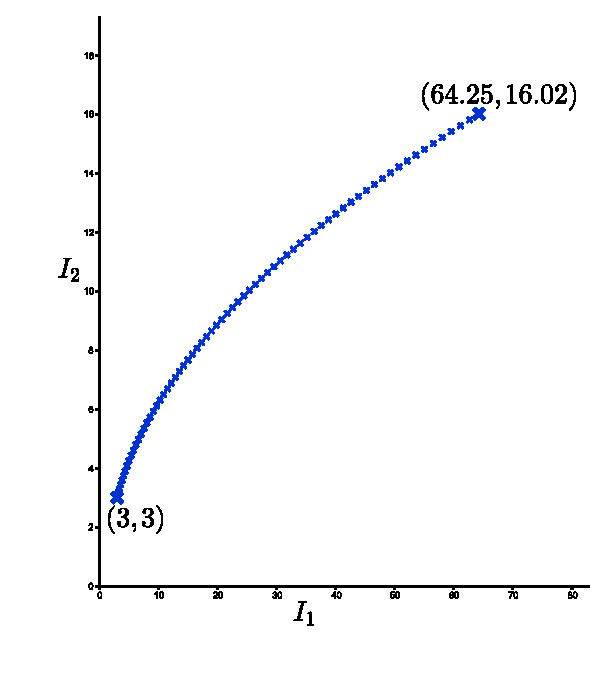
\includegraphics[scale=0.7]{scilab/q2-6-1.eps}
\caption{Traction simple}
\label{fig:tract_simple}
\end{figure}

\subsubsection{Traction plane}
$I_1=\lambda_1^2+1+\dfrac{1}{\lambda_1^2}$ et $I_2=I_1$

\begin{figure}[!ht]
\centering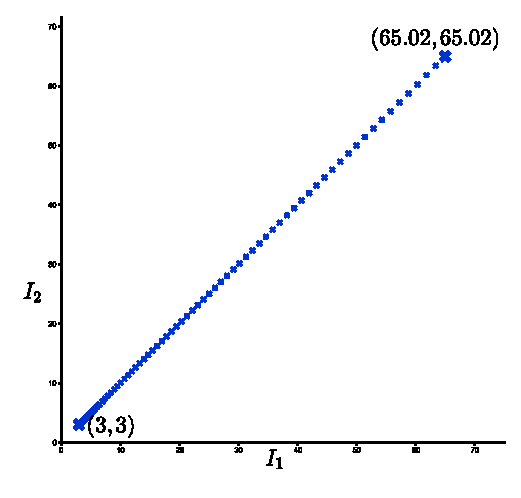
\includegraphics[scale=0.8]{scilab/q2-6-2.eps}
\caption{Traction plane}
\label{fig:tract_plane}
\end{figure}

\newpage
\subsubsection{Traction équibiaxiale}
$I_1=2\lambda_1^2+\dfrac{1}{\lambda_1^4}$ et $I_2=\lambda_1^4+\dfrac{2}{\lambda_1^2}$

\begin{figure}[!ht]
\centering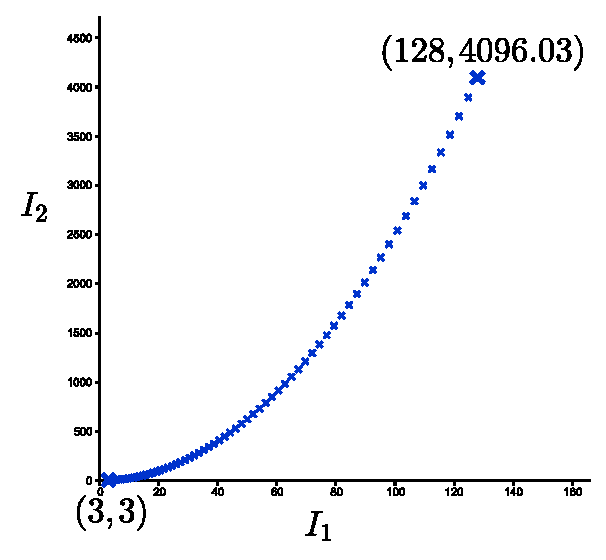
\includegraphics[scale=0.8]{scilab/q2-6-3.eps}
\caption{Traction équibiaxiale}
\label{fig:tract_equi}
\end{figure}

%partie 3
\section{Identification des paramètres de lois NH et de Langevin}

Dans cet exercice, on considère une loi de comportement uniquement caractérisée par le premier invariant : $\psi = \psi(I_1)$.

\subsection {Discussion sur les trois essais}

Dans cette condition, les trois essais nous fournissent les moyens nécessaires pour identifier la forme de la fonction $\frac{\partial\psi}{\partial I_1} (I_1)$ par la mesure les quantités $t_1, t_2, \lambda_1$. L'essai "traction plane" nous permet de calculer $\frac{\partial\psi}{\partial I_1}$ de deux façons indépendantes, c'est-à-dire à partir de $t_1$ ou bien de $t_2$. Toutefois, si l'on ne dispose pas de l'information sur $t_2$, les trois essais sont théoriquement équivalents, étant donné que l'on peut mesurer les quantités $\lambda_1$ et $t_1$ avec une très bonne précision.

\subsection {Traction Simple}
Les équations utilisées pour calculer la quantité $\frac{\partial\psi}{\partial I_1} (I_1(\lambda_1))$ en fonction de $\lambda_1$ supposant $\psi = \psi(I_1)$ sont, d'après le dernier exercice :
\begin{enumerate}
\item[(TS)]
$
\begin{cases}
2 \rho_0 \frac{\partial\psi}{\partial I_1} = \frac{t_1\lambda_1^2}{\lambda^3-1}\\
I_1 = \lambda_1^2 + \frac{2}{\lambda_1}
\end{cases}
$
\item[(TP)]
$
\begin{cases}
2 \rho_0 \frac{\partial\psi}{\partial I_1} = \frac{t_1\lambda_1^3}{\lambda^4-1}\\
I_1 = \lambda_1^2 + 1 + \frac{1}{\lambda_1^2}
\end{cases}
$
\item[(TEB)]
$
\begin{cases}
2 \rho_0 \frac{\partial\psi}{\partial I_1} = \frac{t_1\lambda_1^5}{\lambda^6-1}\\
I_1 = 2\lambda_1^2 + \frac{1}{\lambda_1^4}
\end{cases}
$
\end{enumerate}

\begin{figure}[!ht]
\centering
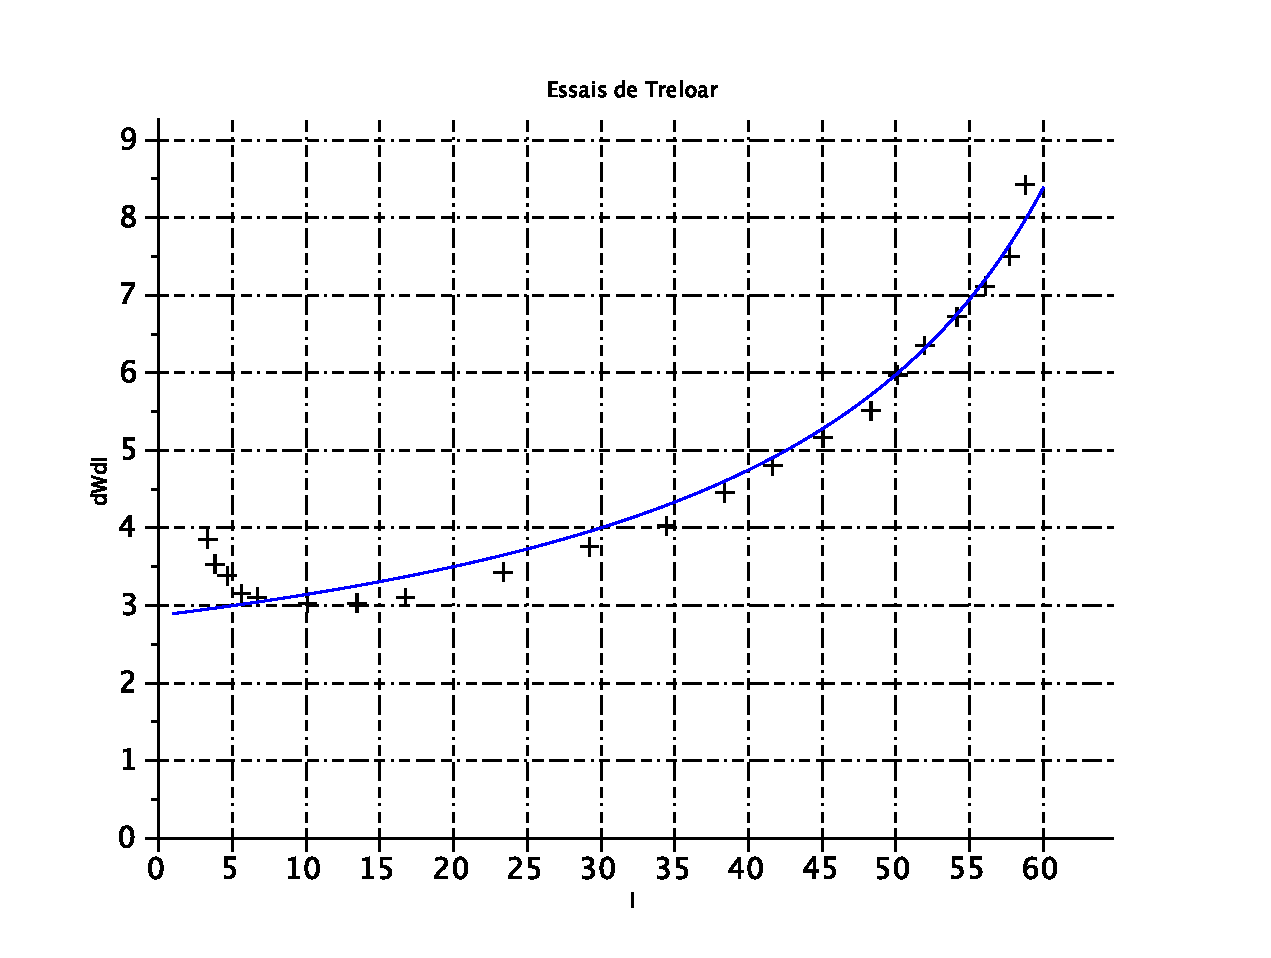
\includegraphics[width=0.7\textwidth]{scilab_prof/q31.pdf}
\caption{Graphe de $2 \rho_0 \frac{\partial\psi}{\partial I_1}$ en fonction de $I_1$ pour l'essai de Traction simple. La courbe bleue répresente la fonction de Langevin avec les paramètres optimaux trouvés dans la question 3 : $C_L = 0.957$ et $N_L=26.9$.}
\label{fig:31}
\end{figure}

La figure \ref{fig:31} contient le graphe paramétrique des relations (TS).

\subsection{Lois NH et de Langevin}
La figure \ref{fig:31} nous indique que les fonctions $\psi$ ont une forte dépendence par rapport premier invariant, surtout quand il dépasse la valeur de $I_1 = 40$. SCILAB nous fournit les outils de régression linéaire et non-linéaire nécessaires pour trouver les paramètres optimaux $C_{NH}$, $C_L$ et $N_L$ dans la régression $2 \rho_0 \frac{\partial\psi}{\partial I_1} = C_{NH}$ (NH) ou $2 \rho_0 \frac{\partial\psi}{\partial I_1} = C_L \frac{9N_L-I_1}{3N_L-I_1}$ (Langevin) (code ci-joint). Les résultats trouvés sont $C_{NH} = 4.73$ et $(C_L, N_L) = (0.957, 26.9)$. Évidemment, pour les grandes valeurs de $I_1$, on a intérêt à utiliser la loi de Langevin, plus appropriée qu'une constante néo-hookéenne dans le domaine d'application de grandes déformations. Pour petites valeurs de $I_1$, la constante optimale devient $C_{NH} \approx 3.5$.

\subsection{TP et TEB - simple dépendence en premier invariant}

On voit dans la figure \ref{fig:32} que la loi de Langevin décrit bien les essais TS et TP. Cependant, l'essai TEB s'écarte des deux autres courbes. On observe que, dans les équations décrivant $t_1$ dans la question 2.6, pour les grandes valeurs de $\lambda_1$, on néglige de plus en plus la dépendence de $\psi$ par rapport à $I_2$ dans l'essai TS. Dans l'essai TP, la valeur de $\frac{\partial\psi}{\partial I_2}$ est déjà pris en compte dans le calcul de $\frac{\partial\psi}{\partial I_1}$. En plus, dans cet essai $I_1 = I_2$. Par contre, dans l'essai TEB, l'écart entre $\frac{\partial\psi}{\partial I_2}$ et $\frac{\partial\psi}{\partial I_1}$ croît avec $\lambda_1^2$, ce qui explique sa courbe dans la figure \ref{fig:32}.

\begin{figure}[!ht]
\centering
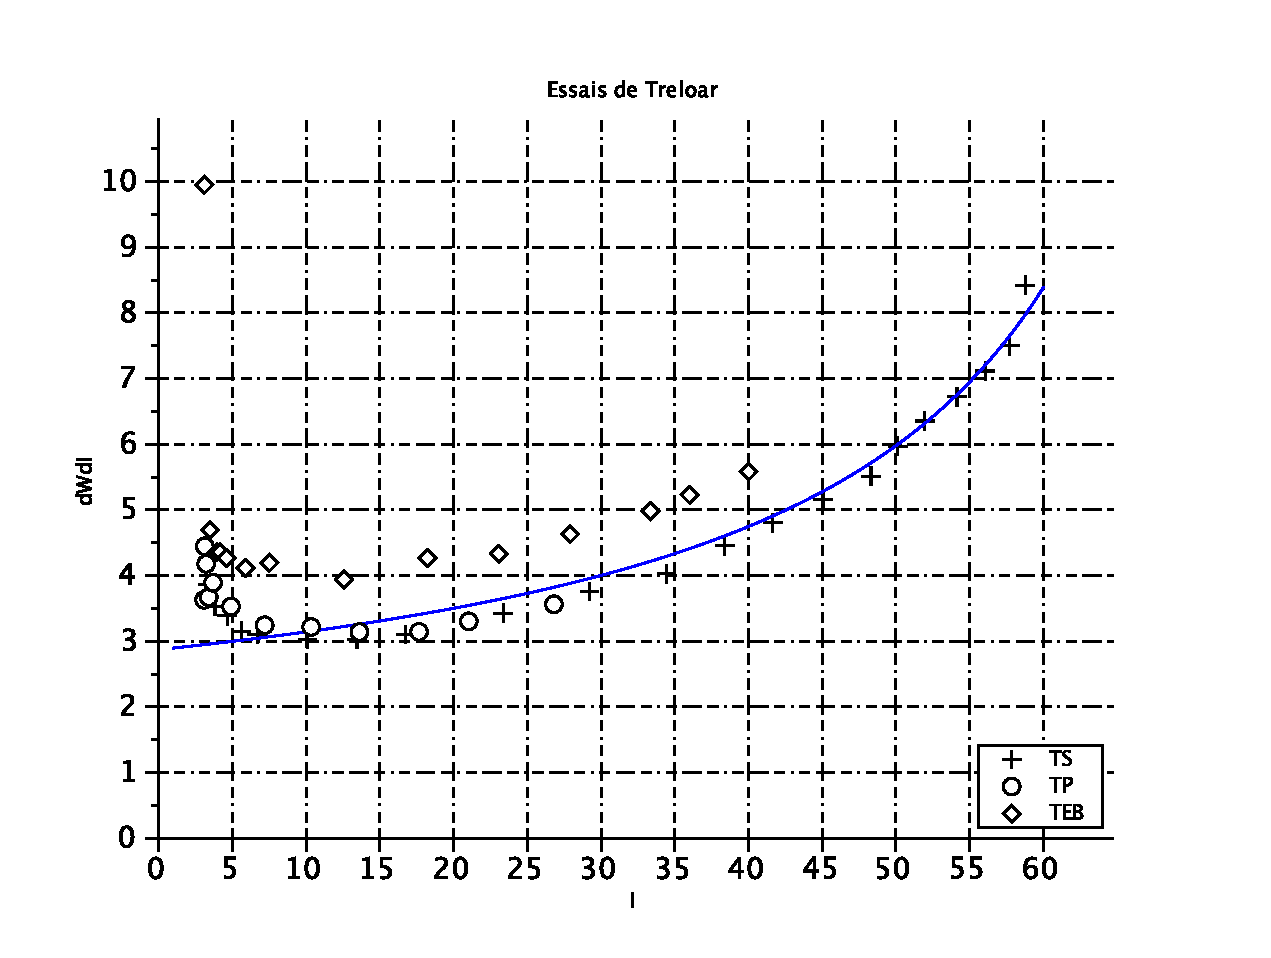
\includegraphics[width=0.6\textwidth]{scilab_prof/q32.pdf}
\caption{Graphe de $2 \rho_0 \frac{\partial\psi}{\partial I_1}$ en fonction de $I_1$ pour tous les essais. La courbe bleue représente la fonction de Langevin avec les paramètres optimaux trouvés dans la question 3 : $C_L = 0.957$ et $N_L=26.9$.}
\label{fig:32}
\end{figure}

%partie 4
\section{Développement d'une loi à deux invariants}
Désormais on rajoute un deuxième terme à la loi de Langevin décrite ci-dessus : $\psi(\tens{e}) = \psi_1(I_1) + \psi_2(I_2)$, avec $\FRAC{\partial\psi}{\partial I_1} = C_L\frac{9N_L-I_1}{3N_L-I_1}$, où les constantes sont celles de la figure \ref{fig:32}. Il s'agit encore d'une simplification, car on néglige les termes croisés $I_1I_2$ ou supérieurs.

\subsection{Dépendence du modèle en deuxième invariant}
On isole $2 \rho_0 \frac{\partial\psi}{\partial I_2}$ dans les équations de la question 2.6 en fonction de $t_1$ et $\lambda_1$. Le résultat est tracé dans les figures \ref{fig:411} à \ref{fig:413}.

\begin{figure}[!ht]
\centering
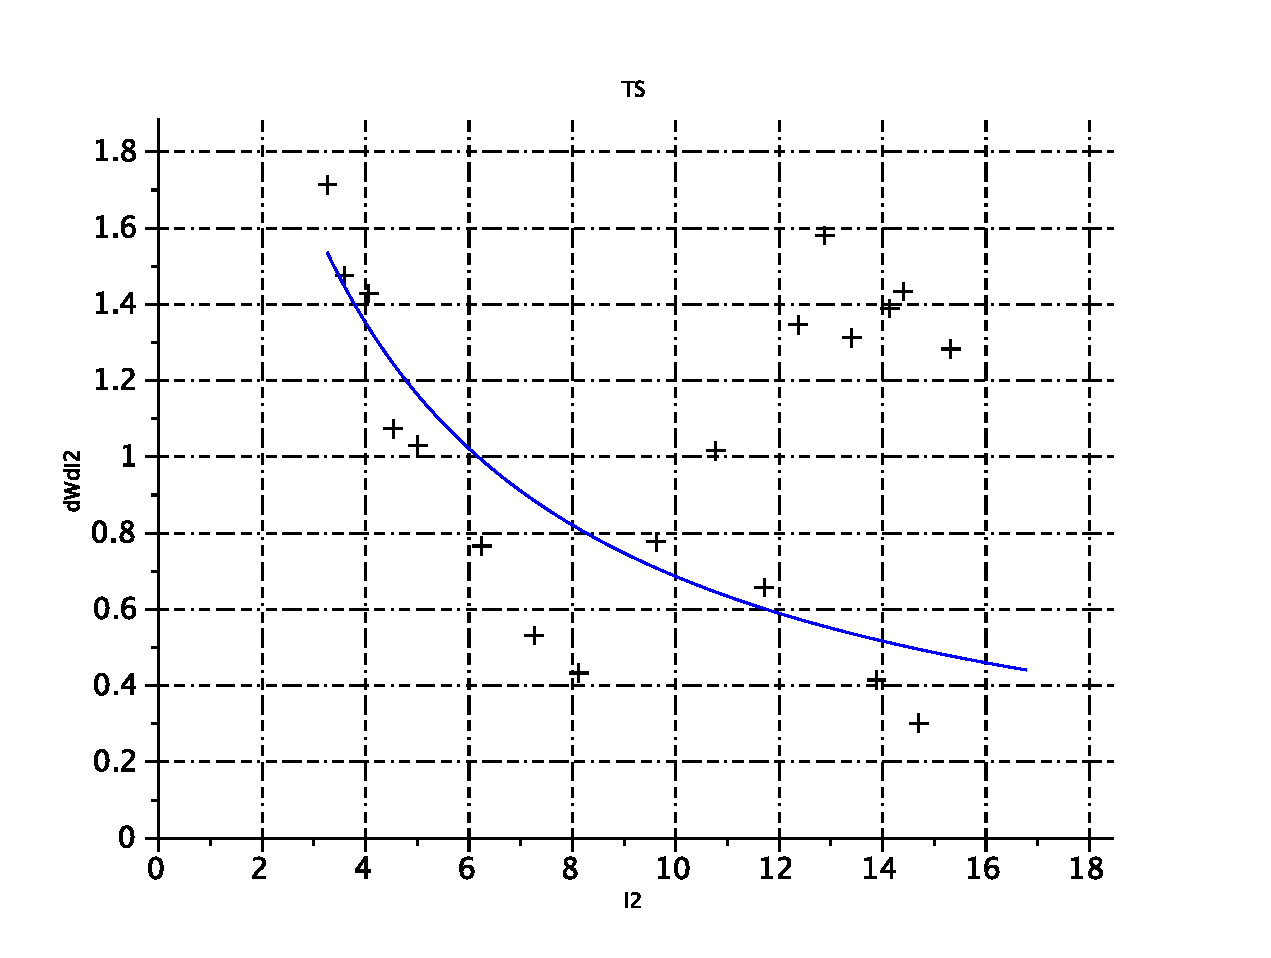
\includegraphics[width=0.5\textwidth]{scilab_prof/q411.pdf}
\caption{Graphe de $2 \rho_0 \frac{\partial\psi}{\partial I_2}$ en fonction de $I_2$ pour l'essai de Traction simple. La courbe bleue représente la régression non-linéaire des données par rapport à une fonction de la forme $A/(I_2-B)$ : $A = 8.37, B = -2.19$.}
\label{fig:411}
\end{figure}
%\begin{figure}[!ht]
%\centering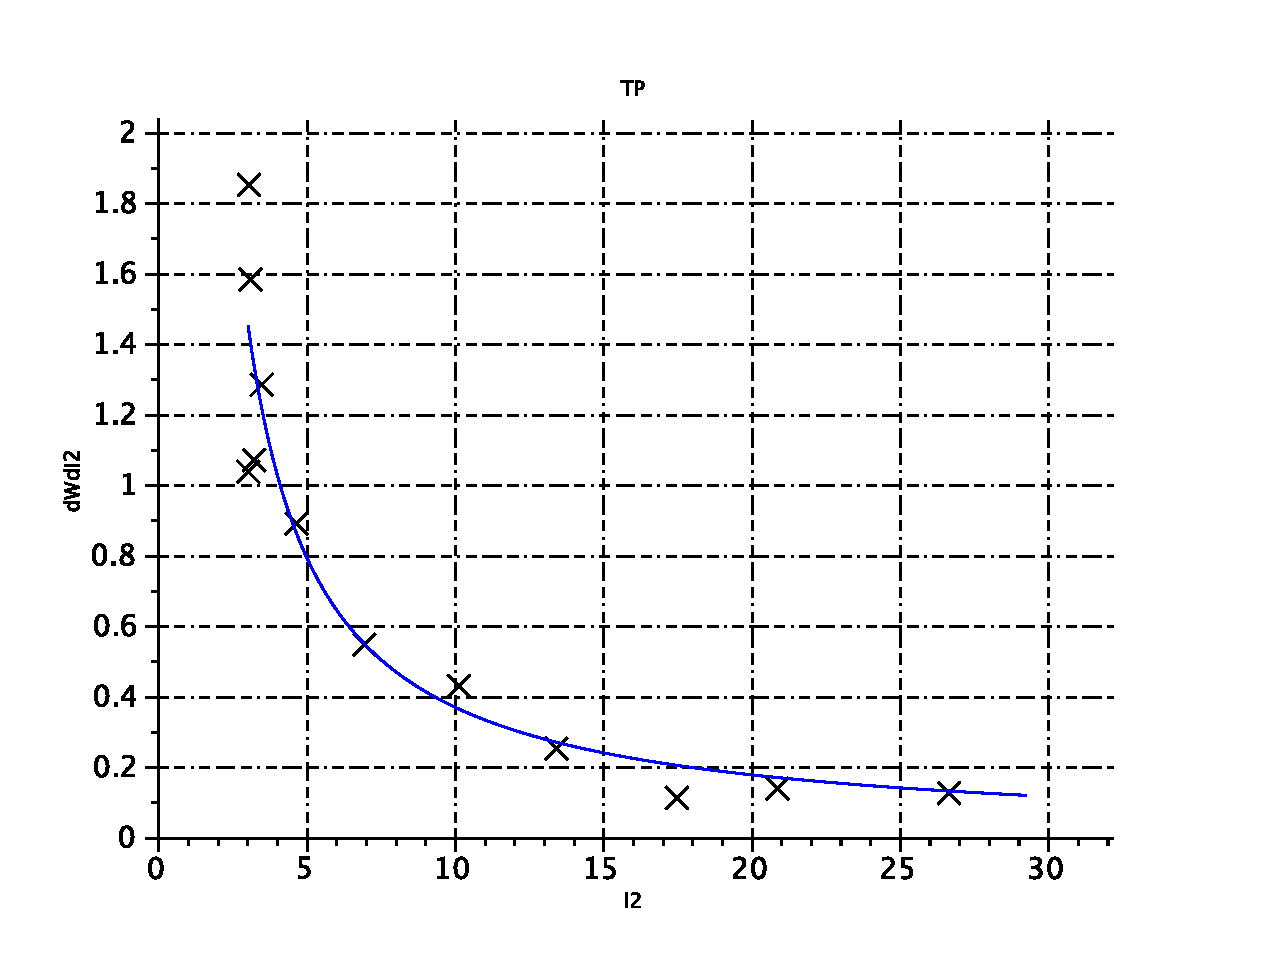
\includegraphics[width=0.4\textwidth]{scilab_prof/q412.pdf}
%\caption{Graphe de $2 \rho_0 \frac{\partial\psi}{\partial I_2}$ en fonction de $I_2$ pour l'essai de Traction plane. La courbe bleue represente la régression non-linéaire des données par rapport à une fonction de la forme $A/(I_2-B)$ : $A = 3.48, B = -0.612$.}
%\label{fig:412}
%\end{figure}
%
%\begin{figure}
%\centering
%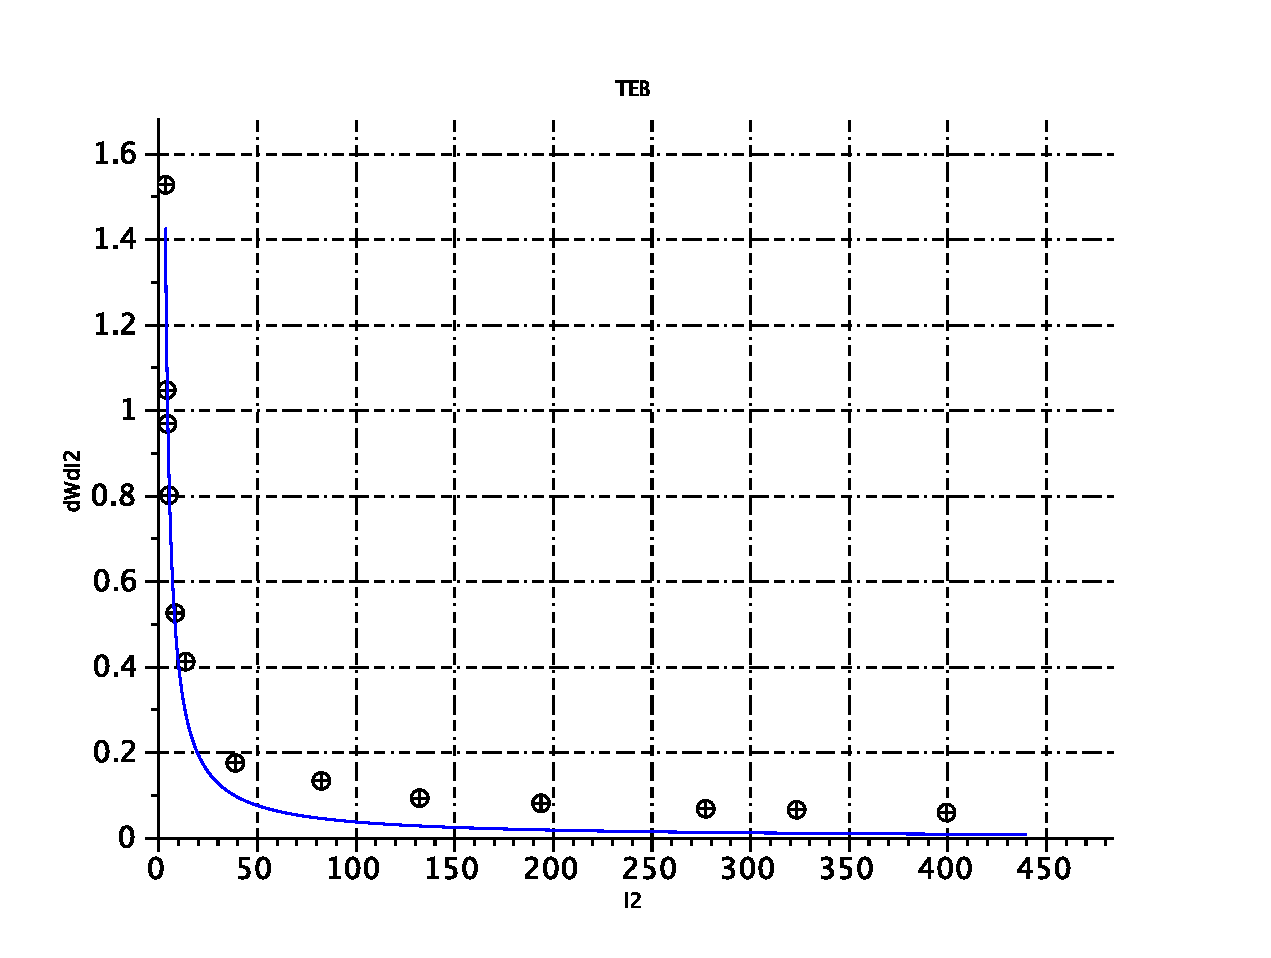
\includegraphics[width=0.7\textwidth]{scilab_prof/q413.pdf}
%\caption{Graphe de $2 \rho_0 \frac{\partial\psi}{\partial I_2}$ en fonction de $I_2$ pour l'essai de Traction équibiaxiale. La courbe bleue représente la régression non-linéaire des données par rapport à une fonction de la forme $A/(I_2-B)$ : $A = 3.77, B = -0.691$.}
%\label{fig:413}
%\end{figure}

\begin{figure}[!h]
\begin{minipage}{0.49\linewidth}
	\centering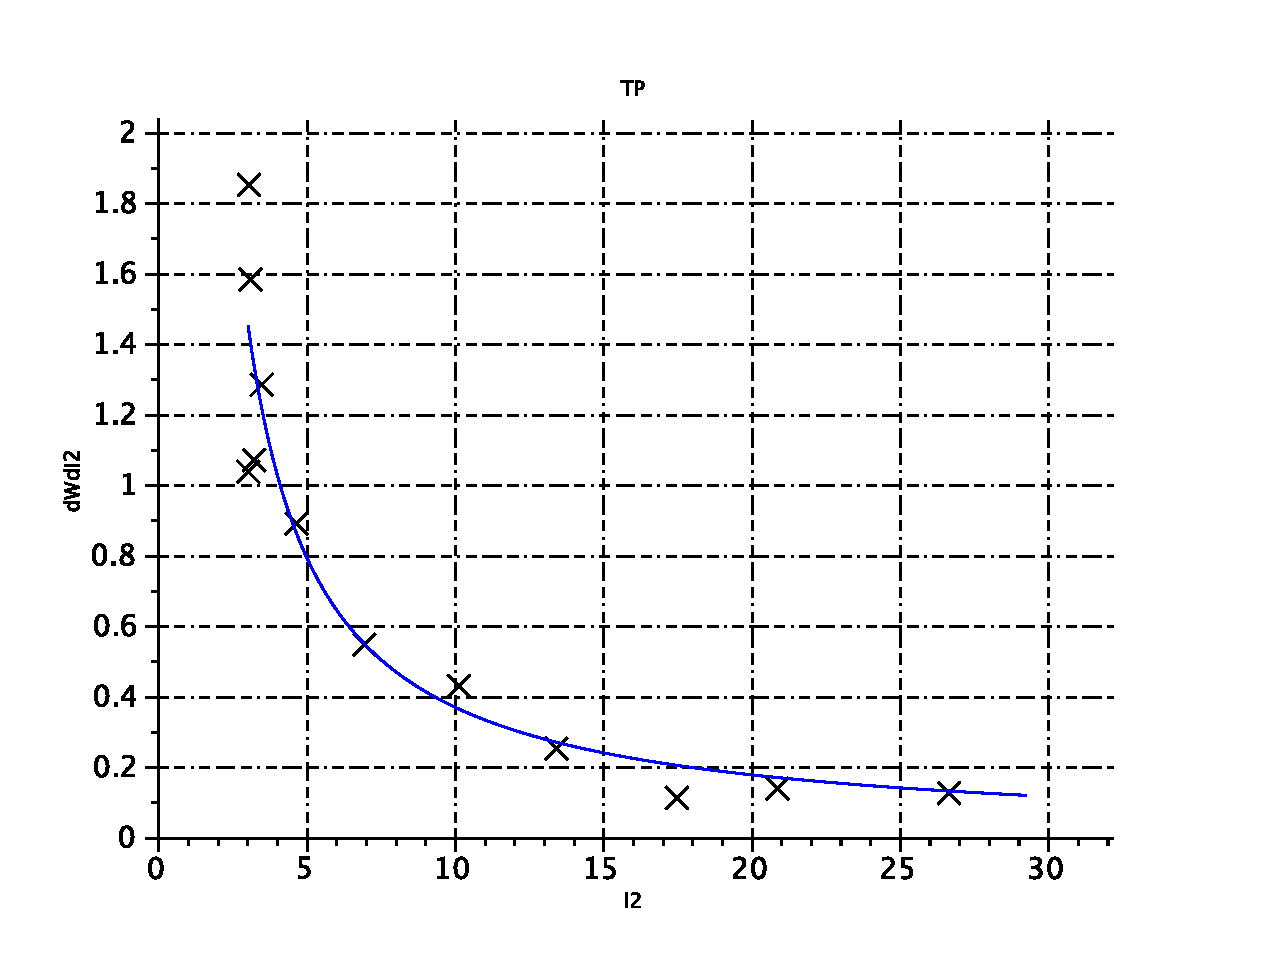
\includegraphics[scale=0.45]{scilab_prof/q412.pdf}
	\caption{Graphe de $2 \rho_0 \frac{\partial\psi}{\partial I_2}$ en fonction de $I_2$ pour l'essai de Traction plane. La courbe bleue represente la régression non-linéaire des données par rapport à une fonction de la forme $A/(I_2-B)$ : $A = 3.48, B = -0.612$.}
\label{fig:412}
\end{minipage}
	\hfill
\begin{minipage}{0.49\linewidth}
	\centering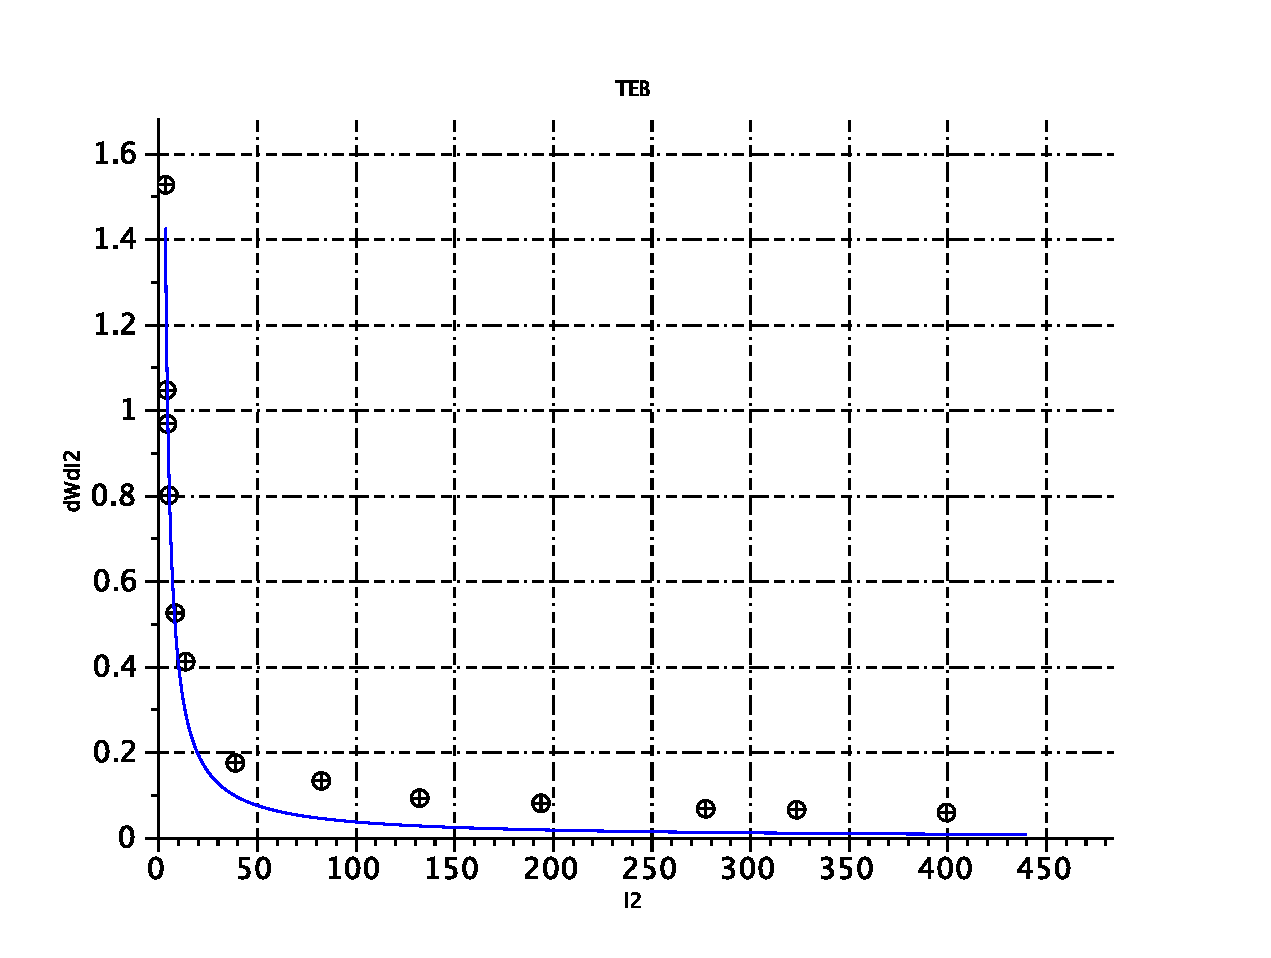
\includegraphics[scale=0.45]{scilab_prof/q413.pdf}
	\caption{Graphe de $2 \rho_0 \frac{\partial\psi}{\partial I_2}$ en fonction de $I_2$ pour l'essai de Traction équibiaxiale. La courbe bleue représente la régression non-linéaire des données par rapport à une fonction de la forme $A/(I_2-B)$ : $A = 3.77, B = -0.691$.}
\label{fig:413}
\end{minipage}
\end{figure}

\FloatBarrier
\subsection{Expression du modèle en fonction du deuxième invariant}
Puisqu'on observe une asymptote en $2 \rho_0 \frac{\partial\psi}{\partial I_2} \rightarrow 0$ et en $I_2 \rightarrow 0$, on choisit une fonction hyperbolique pour la méthode de régression non-linéaire. Ainsi, $2 \rho_0 \frac{\partial\psi}{\partial I_2} = \frac{A}{I_2-B}$ est une fonction candidate. Ici, on négligera la régression trouvée dans l'essai de traction simple, parce que l'ensemble de points ne suit pas une fonction déterminée. On a donc avec une fonction hyperbolique qui prévoit bien l'essai de traction plane, mais dont le comportement est moins adéquat lors de l'essai de traction équibiaxiale pour valeurs de $\lambda_1$ importantes. Ainsi, pour la suite, on prendra comme référence la régression trouvée dans l'essai de TP, c'est-à-dire, $A = 3.48, B = -0.612$.

\subsection{Prévision du modèle enrichi}
Dans la figure \ref{fig:43}, on voit que le modèle prévoit correctement les essais TS et TP. Cependant, on reste toujours avec l'écart entre le modèle et les données réelles pour l'essai TEB à cause du fait que l'on n'a pas réussi à trouver une fonction décrivant aussi bien les phénomènes en TP et TEB.

Il faut reconnaître que même avec cette simplification, on réussit à modéliser les phénomènes en petites déformations ($\lambda_1 < 2$).

%\begin{figure}[!ht]
%\centering
%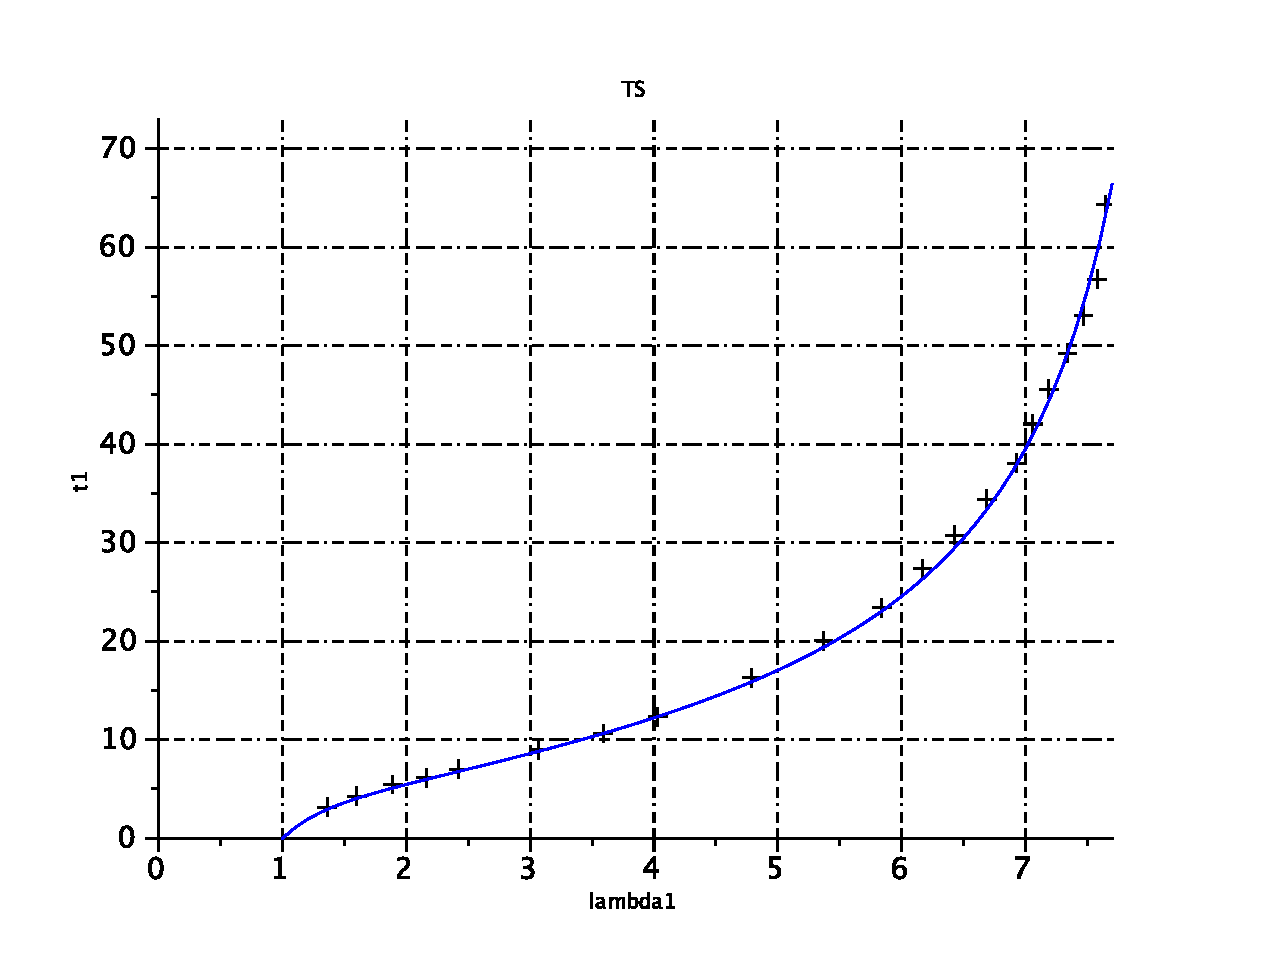
\includegraphics[width=0.6\textwidth]{scilab_prof/q421.pdf}
%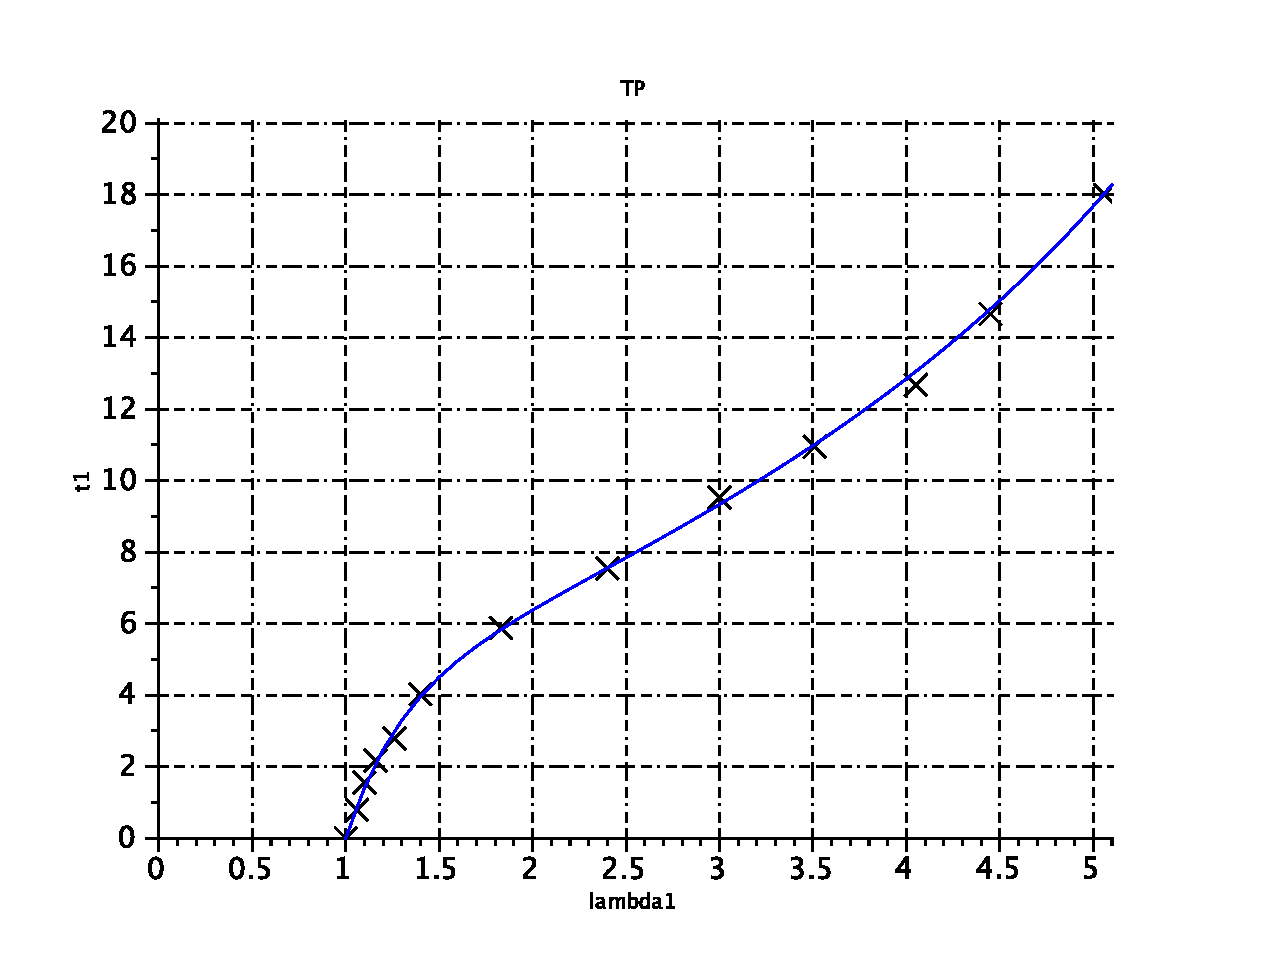
\includegraphics[width=0.6\textwidth]{scilab_prof/q422.pdf}
%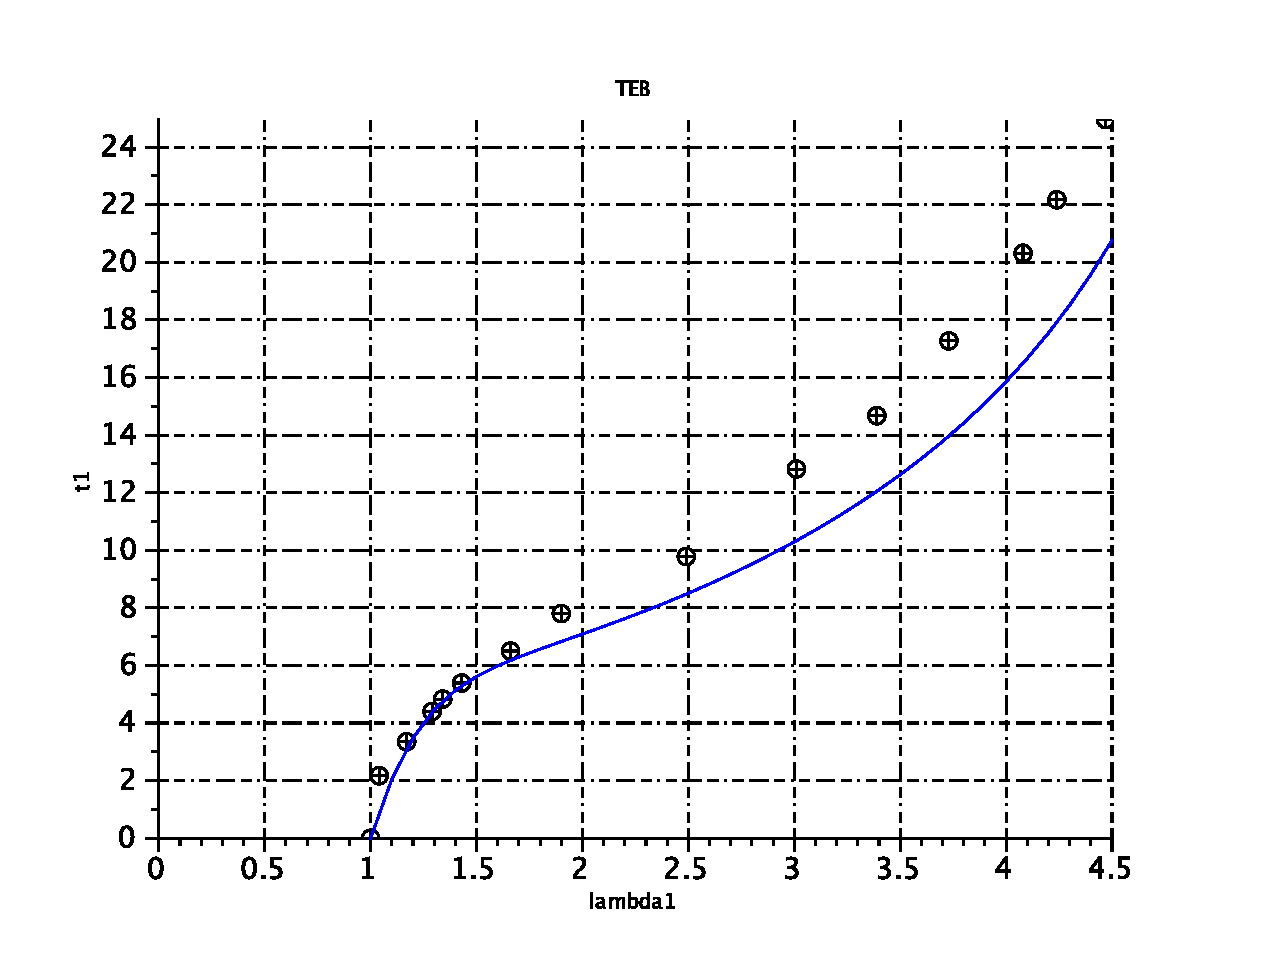
\includegraphics[width=0.6\textwidth]{scilab_prof/q423.pdf}
%\caption{Comparaison entre le modèle de Langevin enrichi et les données réelles pour l'essai TS, TP et TEB.}
%
%\end{figure}

\begin{figure}[!h]
\begin{minipage}{0.49\linewidth}
	\centering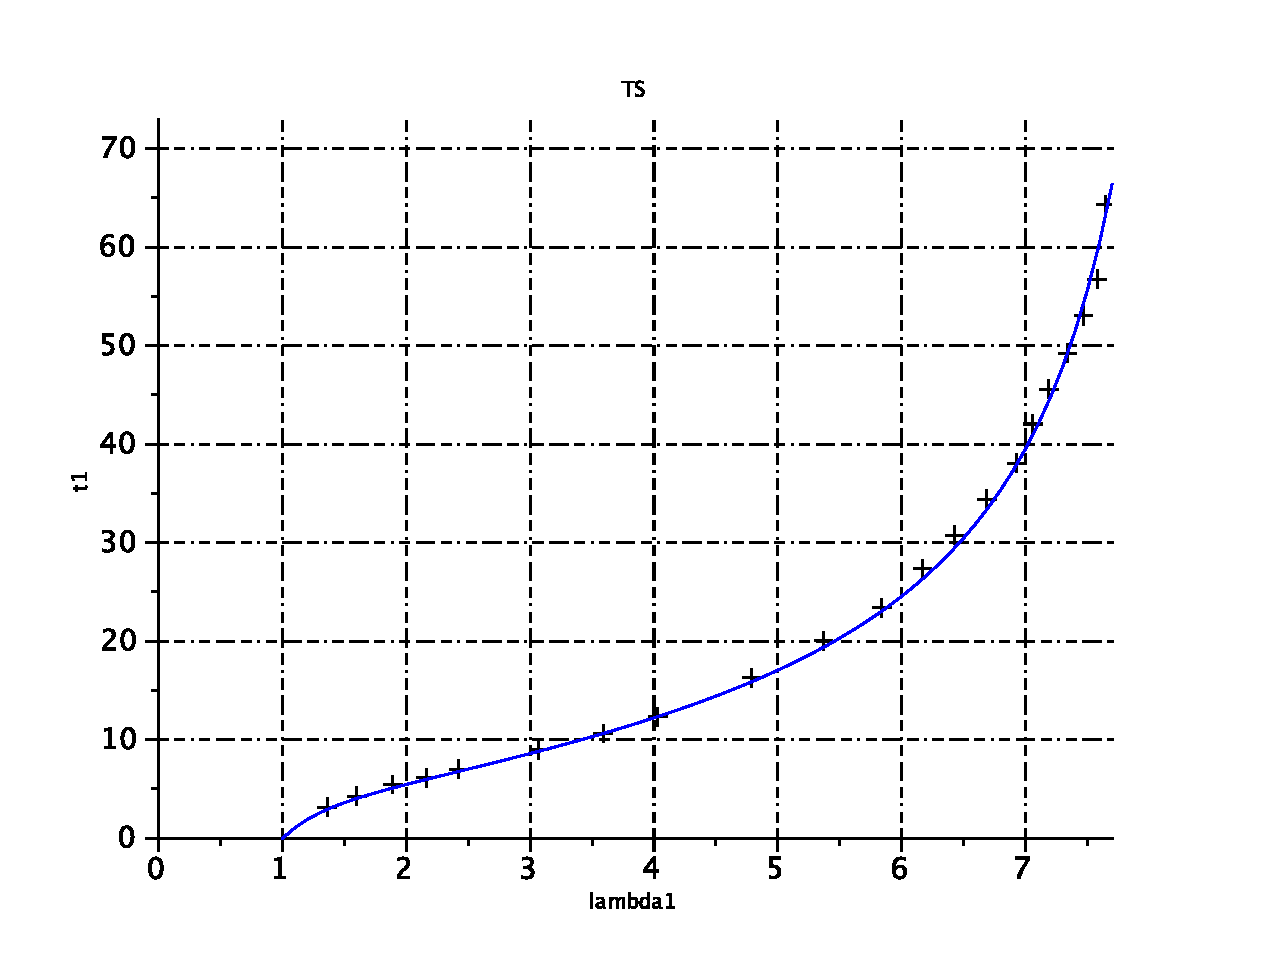
\includegraphics[scale=0.45]{scilab_prof/q421.pdf}
\end{minipage}
	\hfill
\begin{minipage}{0.49\linewidth}
	\centering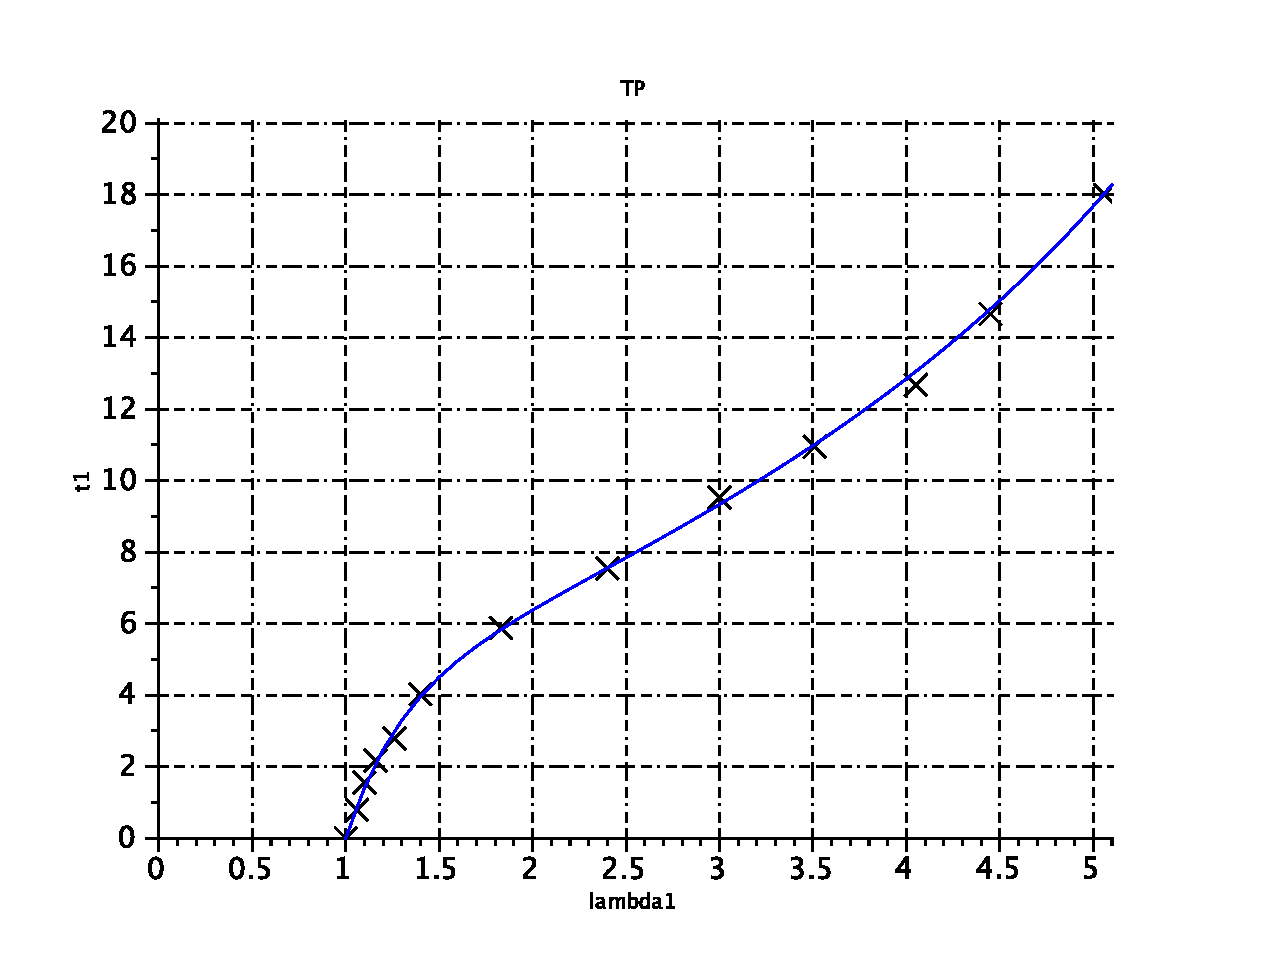
\includegraphics[scale=0.45]{scilab_prof/q422.pdf}
\end{minipage}
\centering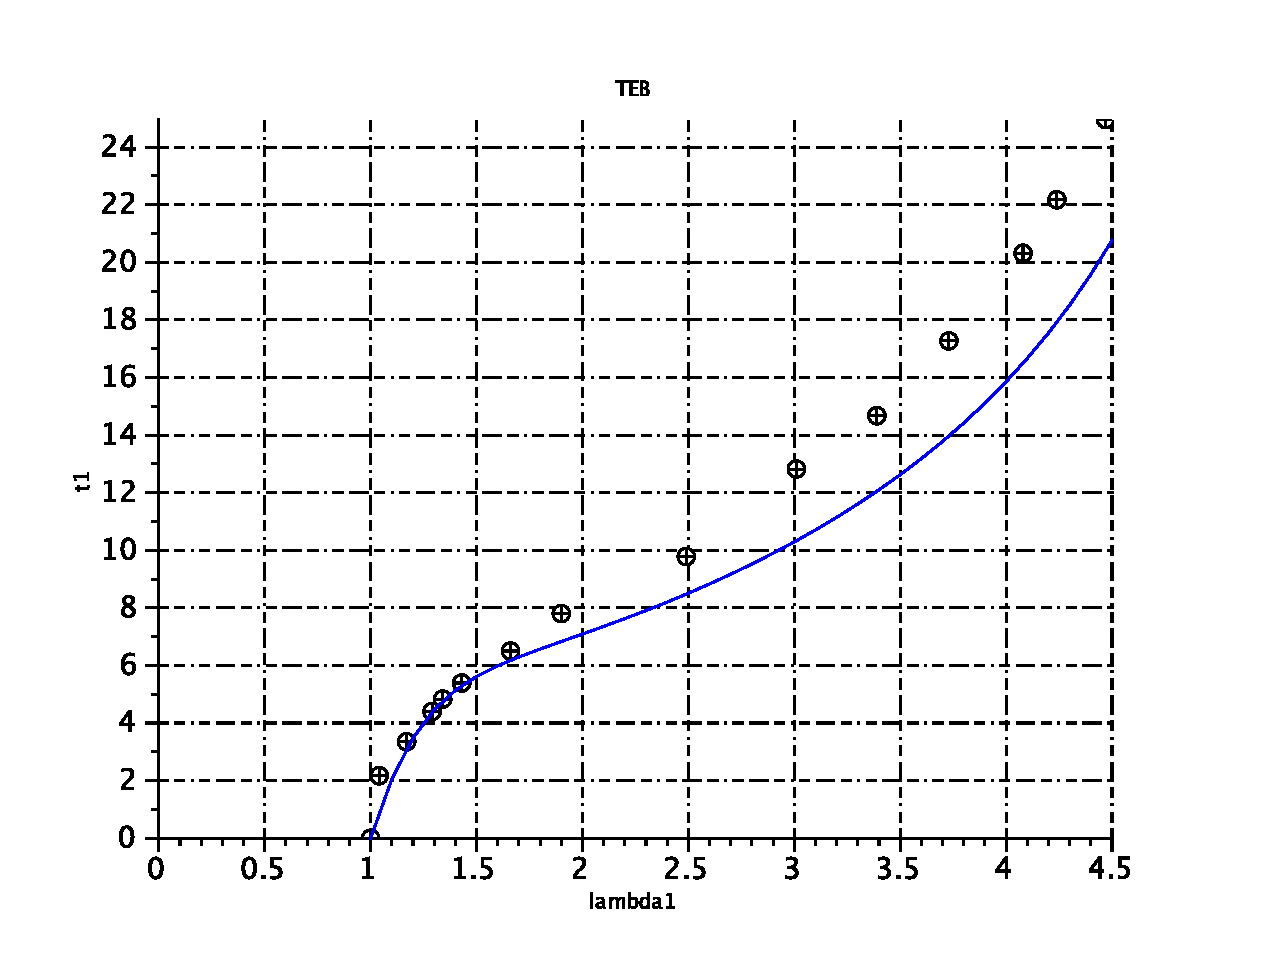
\includegraphics[width=0.6\textwidth]{scilab_prof/q423.pdf}
\caption{Comparaison entre le modèle de Langevin enrichi et les données réelles pour l'essai TS, TP et TEB.}
\label{fig:43}
\end{figure}

\section{Discussion}
\subsection{Décomposition d'un transformation isochore}
Pour un matériau incompressible, on a $det(\tens{F}) = 1$.
Or on peut décomposer $\tens{F} = \tens{R}\cdot \tens{U}$ où :\\
$\tens{R}$ est une rotation qui transforme $(\uline{e'_i})_i en (\uline{e''_i})_i$
$\tens{U} = \SUM_i \lambda_i \uline{e'_i} \otimes \uline{e'_i}$
\\
On a donc :
\begin{align*}
det(\tens{F}) &= \overbrace{det(\tens{R})}^{=1} \cdot det(\tens{U}) \\
&= det(\tens{U}) \\
&= \lambda_1 \lambda_2 \lambda_3 = 1\\
\end{align*}
Soit : $\lambda_3 = \FRAC{1}{\lambda_2 \lambda_1}$ or localement, les $\lambda_i$ sont des constantes donc, par bijections de la fonctions $x \mapsto x^\alpha$, on peut exprimer $\lambda_2$ en fonction de $\lambda_1 = \lambda$ soit : $\lambda_2 = \lambda^\alpha$.

On a donc : $\tens{U} = \lambda \uline{e'_1} \otimes \uline{e'_1} + \lambda^\alpha \uline{e'_2} \otimes \uline{e'_2} + \FRAC{1}{\lambda \lambda^\alpha} \uline{e'_3} \otimes \uline{e'_3}$
De plus : pourquoi lambda>1
$\tens{R}$ étant la rotation qui transforme la base $e'$ en $e''$, on a bien :
\begin{equation}
\fbox{
$
\tens{F} = \lambda \uline{e''_1} \otimes \uline{e'_1} + \lambda^\alpha \uline{e''_2} \otimes \uline{e'_2} + \lambda^{-(\alpha +1)} \uline{e''_3} \otimes \uline{e'_3}
$
}
\end{equation}
On a : $\tens{C} = \trans{\tens{F}} \tens{F} = \trans{\tens{U}} \tens{U}$ car $\tens{R}$ est une rotation.
Par un calcul simple, on obtient :
\begin{align*}
I_1 &= \lambda^2 + \lambda^{2 \alpha} + \lambda^{- 2 (\alpha +1)} \\
I_2 &= \lambda^{-2} + \lambda^{2 (\alpha+1)} + \lambda^{ -2 \alpha} \\
\end{align*}

\begin{figure}[!ht]
\centering\includegraphics[scale=0.5]{scilab/q5-1.eps}
\label{fig:5.1}
\end{figure}

D'après cette figure, le domaine atteignable est l'ensemble des points entre la courbe rouge et la courbe bleu ciel.

\subsection{Comparaison avec la question 2.6 :}
On a donc :
\begin{itemize}
\item Traction simple :
D'après la figure \ref{fig:tract_simple} :  $\alpha = -0.5$
\item Traction plane :
D'après la figure \ref{fig:tract_plane} :  $\alpha = 0$
\item Traction équibiaxiale :
D'après la figure \ref{fig:tract_equi} : $\alpha = 1$
\end{itemize}
Par le tracé précédent, on a donc représenté tout les cas présentés dans la question 2.

On couvre donc l'ensemble des valeurs possibles. Cependant, il manque une ou deux valeurs entre $\alpha = 0$ et $\alpha = 1$ pour avoir le comportement dans cette zone.

\subsection{Résolution pour les trois lois trouvées}
En résolvant le système avec les paramètres optimisés et la loi optimisée trouvées à la partie 3 et 4 on obtient les solutions suivantes:
\begin{figure}[!h]
\centering\includegraphics[scale=0.72]{scilab/q531.eps}
\end{figure}
\begin{figure}[!h]
\centering\includegraphics[scale=0.72]{scilab/q532.eps}
\end{figure}
\FloatBarrier
\clearpage

Points remarquables de la courbe $\Delta p(\lambda)$ :
\begin{itemize}
	\item[Loi NH]
	\begin{enumerate}
	\item $\lambda = 1.6$ maximum local, $\Delta p = 0.118$, en bleu
	\end{enumerate}
	\item[Loi Langevin]
	\begin{enumerate}
	\item $\lambda = 1.6$ maximum local, $\Delta p = 0.039$
	\item $\lambda = 3.7$ minimum local, $\Delta p = 0.027$, en violet
	\end{enumerate}
	\item[Loi Langevin Enrichie]
	\begin{enumerate}
	\item $\lambda = 1.6$ maximum local, $\Delta p = 0.075$
	\item $\lambda = 4.7$ minimum local, $\Delta p = 0.042$, en rouge
	\end{enumerate}
\end{itemize}
\begin{figure}[!h]
\centering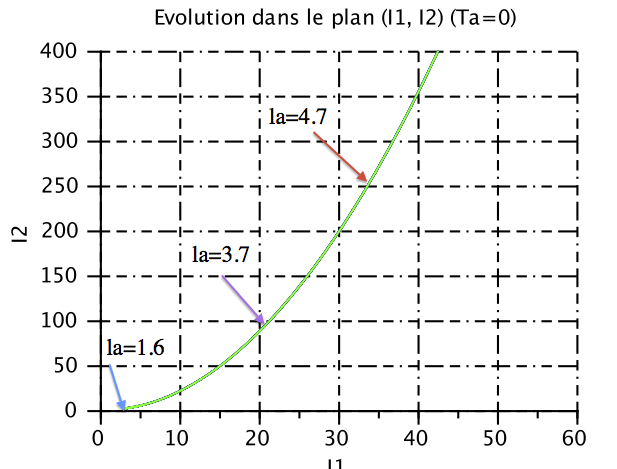
\includegraphics[scale=1.2]{scilab/q533.png}
\end{figure}
\FloatBarrier



\subsection{Cas $T_a$ non-nul}
On observe un décalage des points vers la droite et vers le haut : $\lambda$ et $\Delta p$ plus grands.

\subsection{Conclusion}
Par l'utilisation des paramètres identifiés :
\begin{itemize}
\item Les valeurs de lambda n'ont pas changés
\item La valeur de $\Delta p$ pour la loi NH à augmenté alors que celle pour la loi de Langevin est restée la même
\item On observe la même chose sur les courbes $\Delta p(V/V_ini)$
\end{itemize}

Lorsque $T_a$ est non-nul, on observe un resserrement des courbes pour la loi NH mais pas pour la loi de Langevin.
Avec ces nouveaux coefficients, l'effet de la traction sur la facilité du gonflage devient moindre en considérant les lois de Langevin améliorée et la loi NH. L'absence de changements pour la loi de Langevin est du au fait que la constante choisie est proche de celle proposée à la partie 1.

Comme dans la partie 1, on voit que la loi NH ne diverge pas pour des gonflements importants. Cela pose le problème déjà évoqué dans la première partie.
La loi de Langevin prévoit une divergence du différentiel de pression pour $\lambda=6$ alors que la loi enrichie prévoit une divergence en $\lambda=7$. Cependant, la loi enrichie permet d'expliquer la phase où le gonflage du ballon est facile puisque la courbe est fortement décroissante après $\lambda \approx 2$.

Par le même raisonnement que dans la partie 1, on déduit que la loi enrichie met en avant le fait que tirer sur le ballon facilite le gonflage. En effet, les valeurs de $\mu$ pour $\lambda = 1$ sont plus faibles, le gonflage est donc plus dur relativement aux prévisions de la loi de Langevin.

Pour le départ du gonflage : la loi NH et de Langevin enrichie prévoient bien une forte difficulté du gonflage alors que la loi de Langevin ne le prévoit pas (3 fois moins de difficulté que la loi NH par exemple).
Pour la suite, où le gonflage est plus facile, la loi NH et de Langevin enrichie prévoient toutes deux la facilité observée.
Enfin, lorsque le ballon commence à être très gonflé, les lois Langevin et de Langevin enrichie prévoient toutes deux la divergence du différentiel de pression ce qui correspond mieux à la réalité.
En conclusion, on peut faire confiance à la loi de Langevin enrichie sur tout le domaine, au moins en terme de comportement. Puisque la courbe $(I_1, I_2)$ du gonflage s'approche mieux à celle de l'essai TEB (figure \ref{fig:tract_equi}), d'après la figure \ref{fig:43}, on voit que l'on ne peut pas faire confiance aux valeurs précises de $\Delta p$ à partir de $I_1 > 8$, c'est-à-dire à partir de $\lambda \approx 2.5$.

Les sollicitations pour les essais en traction simple, plane et équibiaxiale sont respectivement de 8, 5 et 4.5 or on a représenté les courbes de gonflage pour $\lambda \in [1, 7]$. Cependant, dans l'essai de la traction simple la régression linéaire n'a pas donnée de résultat satisfaisant et donc doit être écarté. De fait, on doit se limiter à $\lambda = 5$, d'où les courbes représentées sont surement très approximatives pour des valeurs de $\lambda$ supérieures à 6.

On pourrait proposer un essai de traction qui respect la géométrie du problème. En effet, on peut imaginer un test semblable au test de traction équibiaxiale mais en géométrie cylindrique : un anneau attaché au ballon qui changerait de diamètre.




%appendice éventuel
%\clearpage
%\rhead{Annexe}
%\renewcommand{\appendixpagename}{\centering{Annexe : Liste des fonctions Scilab}}
%\renewcommand{\labelitemi}{$\bullet$}
%\renewcommand{\labelitemiii}{$\cdot$}
%\renewcommand{\labelitemii}{$\diamond$}
%\renewcommand{\labelitemiv}{$\ast$}
%\begin{appendices}
%\end{appendices}
\end{document}
